\documentclass[]{book}
\usepackage{lmodern}
\usepackage{amssymb,amsmath}
\usepackage{ifxetex,ifluatex}
\usepackage{fixltx2e} % provides \textsubscript
\ifnum 0\ifxetex 1\fi\ifluatex 1\fi=0 % if pdftex
  \usepackage[T1]{fontenc}
  \usepackage[utf8]{inputenc}
\else % if luatex or xelatex
  \ifxetex
    \usepackage{mathspec}
  \else
    \usepackage{fontspec}
  \fi
  \defaultfontfeatures{Ligatures=TeX,Scale=MatchLowercase}
\fi
% use upquote if available, for straight quotes in verbatim environments
\IfFileExists{upquote.sty}{\usepackage{upquote}}{}
% use microtype if available
\IfFileExists{microtype.sty}{%
\usepackage{microtype}
\UseMicrotypeSet[protrusion]{basicmath} % disable protrusion for tt fonts
}{}
\usepackage[margin=1in]{geometry}
\usepackage{hyperref}
\hypersetup{unicode=true,
            pdftitle={Continuous Classification using Deep Neural Networks},
            pdfauthor={Nick Strayer},
            pdfborder={0 0 0},
            breaklinks=true}
\urlstyle{same}  % don't use monospace font for urls
\usepackage{natbib}
\bibliographystyle{apalike}
\usepackage{longtable,booktabs}
\usepackage{graphicx,grffile}
\makeatletter
\def\maxwidth{\ifdim\Gin@nat@width>\linewidth\linewidth\else\Gin@nat@width\fi}
\def\maxheight{\ifdim\Gin@nat@height>\textheight\textheight\else\Gin@nat@height\fi}
\makeatother
% Scale images if necessary, so that they will not overflow the page
% margins by default, and it is still possible to overwrite the defaults
% using explicit options in \includegraphics[width, height, ...]{}
\setkeys{Gin}{width=\maxwidth,height=\maxheight,keepaspectratio}
\IfFileExists{parskip.sty}{%
\usepackage{parskip}
}{% else
\setlength{\parindent}{0pt}
\setlength{\parskip}{6pt plus 2pt minus 1pt}
}
\setlength{\emergencystretch}{3em}  % prevent overfull lines
\providecommand{\tightlist}{%
  \setlength{\itemsep}{0pt}\setlength{\parskip}{0pt}}
\setcounter{secnumdepth}{5}
% Redefines (sub)paragraphs to behave more like sections
\ifx\paragraph\undefined\else
\let\oldparagraph\paragraph
\renewcommand{\paragraph}[1]{\oldparagraph{#1}\mbox{}}
\fi
\ifx\subparagraph\undefined\else
\let\oldsubparagraph\subparagraph
\renewcommand{\subparagraph}[1]{\oldsubparagraph{#1}\mbox{}}
\fi

%%% Use protect on footnotes to avoid problems with footnotes in titles
\let\rmarkdownfootnote\footnote%
\def\footnote{\protect\rmarkdownfootnote}

%%% Change title format to be more compact
\usepackage{titling}

% Create subtitle command for use in maketitle
\newcommand{\subtitle}[1]{
  \posttitle{
    \begin{center}\large#1\end{center}
    }
}

\setlength{\droptitle}{-2em}
  \title{Continuous Classification using Deep Neural Networks}
  \pretitle{\vspace{\droptitle}\centering\huge}
  \posttitle{\par}
  \author{Nick Strayer}
  \preauthor{\centering\large\emph}
  \postauthor{\par}
  \predate{\centering\large\emph}
  \postdate{\par}
  \date{2017-12-08}

\usepackage{booktabs}
\usepackage{amsthm}
\makeatletter
\def\thm@space@setup{%
  \thm@preskip=8pt plus 2pt minus 4pt
  \thm@postskip=\thm@preskip
}
\makeatother

\usepackage{amsthm}
\newtheorem{theorem}{Theorem}[chapter]
\newtheorem{lemma}{Lemma}[chapter]
\theoremstyle{definition}
\newtheorem{definition}{Definition}[chapter]
\newtheorem{corollary}{Corollary}[chapter]
\newtheorem{proposition}{Proposition}[chapter]
\theoremstyle{definition}
\newtheorem{example}{Example}[chapter]
\theoremstyle{definition}
\newtheorem{exercise}{Exercise}[chapter]
\theoremstyle{remark}
\newtheorem*{remark}{Remark}
\newtheorem*{solution}{Solution}
\let\BeginKnitrBlock\begin \let\EndKnitrBlock\end
\begin{document}
\maketitle

{
\setcounter{tocdepth}{1}
\tableofcontents
}
\chapter{Introduction}\label{intro}

\section{Continuous Classification}\label{continuous-classification}

Imagine you are watching a movie. A friend walks in late and asks ``what
did I miss?'' You tell them the main character has just escaped from a
nasty predicament and has defeated the antagonist. What you have done is
classification on a sequence. The sequence in this case is the frames of
the movie and your classification was what was occurring in the movie at
that moment. You \emph{could} have given the same answer if you just saw
a single frame, but most likely your assessment of the state of the
movie depended on events you saw before and the context in which they
placed the most recent frame.

Continuous classification in the context of statistics and machine
learning is training models to observe data over time, like you watched
the movie, and classify the status of the generating system at any given
point. Sometimes seeing the most recent data is all that is needed, but
more interesting and challenging problems need the algorithm to be able
to make decisions about a current time while leveraging context from
previous history to do so.

This report is a brief run through past attempts at continuous
classification and a deeper exploration of the current state of the art
methods.

\section{Potential applications of continuous classification
models}\label{potential-applications-of-continuous-classification-models}

The following are just a few examples of biomedical applications made
possible with effective continuous classification models.

\subsection{Activity Prediction}\label{activity-prediction}

With the advent of wearable devices such as fitbits and apple watches,
the amount of high temporal resolution data we have streaming from
individuals is exploding and showing no sign of letting up.

Continuous classification models could use these data to classify the
state of the wearer at any moment. A simple example of this is detecting
different exercise types (e.g.~running vs.~swimming); which is
implemented (by unpublished methods) internally at companies such as
fitbit.

More advanced, and potentially impactful, applications include extending
the predictions to more subtle but medically relevant states such as
dehydration or sleep apnea (\citet{wearable_atrial}). Preliminary work
in these areas using deep learning has shown surprising success with
data as limited as heart-rate and motion indication being enough to
predict sleep apnea and various cardiovascular risk states with a
c-statistic of 0.94: comparable to invasive gold standards.

\subsection{EHR monitoring}\label{ehr-monitoring}

With more and more information on patients being accrued in government
and hospital databases we have a clearer than ever picture of a
patient's health over long periods of time. Unfortunately, due to a
combination of overwhelming quantities and noise levels in the data, our
ability to make use of these data has not kept up with their quantity.

Sequential models can help ease the burden on health practitioners in
making use of these data. For instance, a model could be trained on a
patient's records to predict the likelihood of cardiovascular events.
This model could then alert a doctor of potential risk in order to
facilitate timely interventions. This could be especially helpful in
large clinical settings where personal doctor-patient relationships may
not be common. For a review of the performance of deep learning models
in electronic health record contects, see \citet{deep_ehr}.

\subsection{Hospital Automation}\label{hospital-automation}

Patient monitoring systems already have alarms to alert staff of
occurring anomaly for a patient. Continuous classification methods could
extend these systems to warn \emph{before} the anomaly occurs
(e.g.~patient has a high change of going into afribulation in the next
five mins), or to more subtle actions (patient is experiencing pain and
needs a change in the medications administered by their IV). These
methods, if successfully implemented could help hospitals more
efficiently allocate resources and potentially save lives.

\section{History of methods}\label{history-of-methods}

While sources of data well suited to it have recently greatly expanded,
interest in performing continuous classification is not a new topic.
Many methods have been proposed for the task to varying degrees of
success. Below is a brief review of some of the more successful methods
and their advantages and limitations.

\subsection{Windowed regression}\label{windowed-regression}

Perhaps the most intuitive approach to the problem of incorporating
context from previous time points into your prediction is to use a
windowed approach. Broadly, in these approaches a window of some width
(in previous observation numbers or time length) is sequentially run
over the series. The data obtained from the window may have some form of
summary applied to it. This could be a mean, median, or any other
function which is then used to predict with.

By summarizing the multiple data-points into a single (or few) values
noise can be removed, but at the cost of potentially throwing away
useful information captured by the interval (such as trajectory.)

If the data are kept intact more advanced methods are available. These
include dynamic time warping (\citet{dtw}) or kernel methods (see next
section). This allows more information to be retained in the sample but
at the cost of setting a limit on how far back your model can learn
dependencies in the data. For instance, if your window is one hour long
but an activity lasts two hours your model will have a very hard time
recognizing it. This is equivalent to an infinitely strong prior on the
interaction timeline (\citet{graves_rnn}).

\subsection{Transformation methods}\label{transformation-methods}

As mentioned before, when a window is scanned across the time dimension
of data, one of the ways of extracting information is by performing some
transformation on the data. Common examples include wavelet or Fourier
transforms. These methods attempt to separate the data into separate
components. For instance, Fourier transforms applied to accelerometer
data from an individuals wrist can be used to detect the frequencies
associated with walking and running (\citet{accelerometer_activity}).
These methods have also been used extensively in electrical systems and
signal processing to help determine the state of the system.

\begin{figure}

{\centering 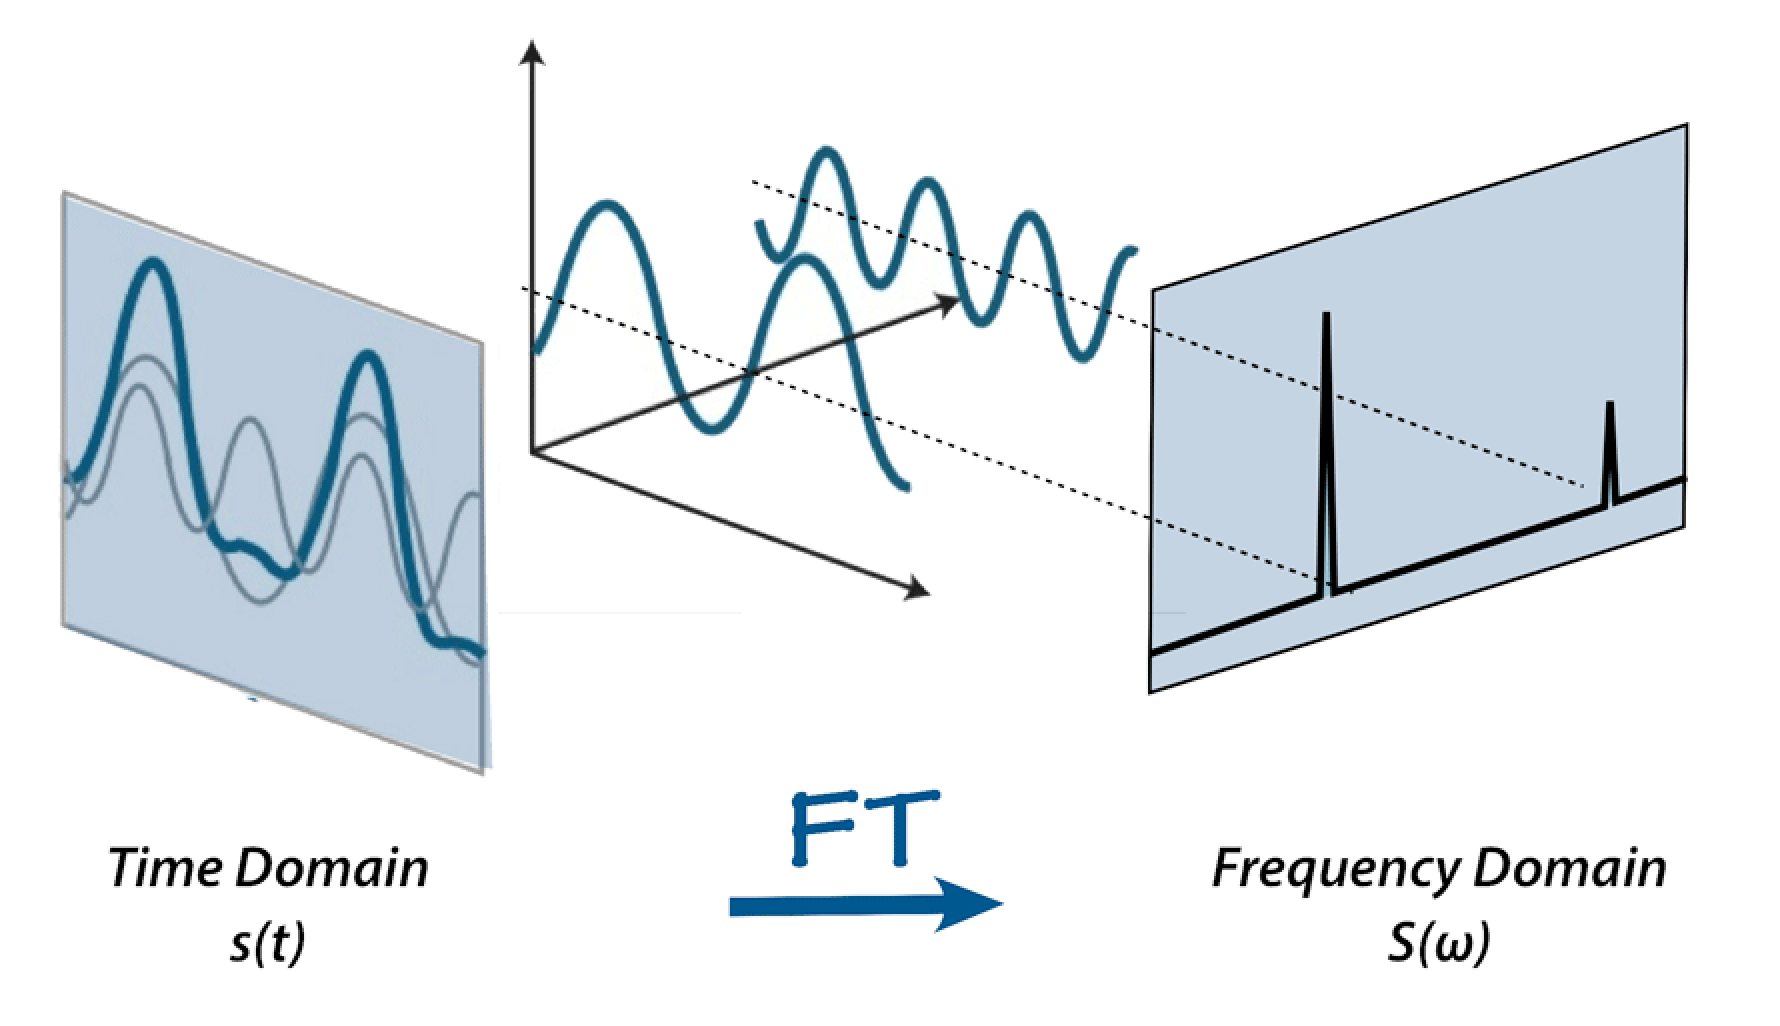
\includegraphics[width=0.6\linewidth]{figures/fourier_transform} 

}

\caption{Example of transforming data from the data-domain to the frequency-domain for time series data. Image courtousy of [Allen D. Elster, MD FACR](http://mriquestions.com/index.html).}\label{fig:fouriertransform}
\end{figure}

A few limitations are imposed by these methods. First, as previously
mentioned, they are subject to the windowing constraints. Secondly, they
rely on the data to be periodic or oscillatory in nature. For instance,
accelerometer data oscillates back and forth as the individual swings
their arms and electrical systems are inherently oscillatory. Data such
as heart-rate or step counts produced by devices like apple watches and
fitbits are a rather stable signal \footnote{Although the raw data the
  sensors receive may not be.} and thus transformation methods are
unable to separate them into frequency domains at small time scales. In
addition, these methods are unable to deal with non-numeric data which
severally limits them in heterogeneous data domains such as EHR data.

\subsection{Hidden Markov Models}\label{hidden-markov-models}

In an attempt to deal with the fact that in most scenarios the
classification of time point \(t\) is dependent on that of previous time
points, hidden Markov models (or HMMs) model data as a series of
observations generated by a system transitioning between some unobserved
(or latent) states. This is done by constructing a transition matrix
that denotes the probability of transitioning from one state to another
and conditioning it on whatever observed data you have.

\[P(s_a -> s_b | x_t) = ...\]

This allows the model to learn time dependencies in the data. For
instance, if a person is running now their next state is probably going
to be walking rather than sitting or swimming.

HMMs were the state of the art models on continuous classification
problems until very recently and are still very valuable for many
problems. However, their greatest advantage is also their greatest
disadvantage.

The Markov property (or the first `M' in HMM) states that the next state
of the system being modeled depends exclusively on the current state.
This means that the model is `memory-less.' For instance, returning to
our running example, say an individual had been running in the previous
time point, the model will most likely pick walking as their next state
(ignoring any conditional data for simplicity) but what if before they
were running they were swimming? This fact from multiple time-steps
before would strongly hint that the next state would in fact be biking
and not walking (they are running a triathlon.)

There are ways to fix this such as extending the model's transition
probabilities to multiple time-steps, however the number of parameters
needed to estimate transition probabilities for \(m\) previous time
steps is (\# of classes) to the \(k^{th}\) power, which rapidly becomes
untenable. In addition, we have to a priori decide the number of time
steps in the past that matter.

\subsection{Advantages of deep learning
methods}\label{advantages-of-deep-learning-methods}

Before we dive into the mathematical underpinnings of deep learning
methods we will go over how they solve many of the aforementioned issues
from traditional methods.

\subsubsection{Less Domain Knowledge
Needed}\label{less-domain-knowledge-needed}

One of the ways that it helps to think about deep learning is as a
computer program that programs itself given an objective and examples.
In his popular blog post
\href{https://medium.com/@karpathy/software-2-0-a64152b37c35}{\emph{Software
2.0}} Andrej Karapathy makes the argument that deep learning is powerful
because it helps avoid traditionally tedius processes like explicitly
defining cases for the computer to deal with. One of the ways this is
applicable to our problems is the ability for deep learning models to
adapt to a wide range of problem/ data domains without much
human-defined customization.

This can be seen in the context of the input data form. If you had data
from an accelerometer it could be fit into the same neural network as
data from a more static heart-rate sensor would. The models are flexible
enough to learn how to deal with these input patterns without requiring
the researcher to explicitly define a transformation based on the data.
One advantage of this independence from large amounts of human
intervention has the potential to make performance assessments more
accurate (\citet{rms}).

\subsubsection{Can find and deal with arbitrary time
dependencies}\label{can-find-and-deal-with-arbitrary-time-dependencies}

Deep learning models are theoretically capable of learning time
dependencies of infinite length and strength
(\citet{universal_approximators}). While obviously it is impossible to
supply a network with enough data to fit the number of parameters
neccesary to do so, the fact remains that deep learning methods are
capable of handling long-term time dependencies. In addition to being
able to model these dependencies they do so without any need for
explicitly telling the model the length of the dependencies and also
using substantially fewer parameters than an extended hidden Markov
model (\citet{graves_rnn}).

For example, a recurrent neural network (RNN) can automatically learn
that if a person swims and then runs, they will most likely be biking
next, but it could also remember that a patient was given a flu vaccine
three months prior and thus their symptoms most likely don't indicate
the flu but a cold. This flexibility to automatically learn arbitrary
time dependency patterns is powerful in not only its ability to create
accurate models, but potentially for exploration of causal patterns.

\subsubsection{Multiple architectures for solving traditional
problems}\label{multiple-architectures-for-solving-traditional-problems}

In a similar vein, one of the decisions that does need to be made with
deep learning: which network architecture to use, conveniently is rather
robust to the problem of continuous classification. For instance:
convolutional neural networks that have achieved great success in
computer vision were actually originally designed for time series data,
and recent advanced such as dilated convolutions
(\citet{dilated_convolutions}) allow for them to search as far back in
the time-series as needed to find valuable information for
classification. Recurrent neural networks (which will be elaborated on
in the following sections) are also fantastic for time-series data, as
they explicitly model the autocorrelation found in the data via a
recurrent cycle in their computation graph. This allows them to read
data much like one reads a book, selectively remembering past events
that have applicability to the current state.

\subsubsection{Downsides}\label{downsides}

As a result of being so flexible deep learning models require a lot of
data to properly tune all their parameters without over fitting. This
results in not only more data being needed (with some exceptions such as
Bayesian methods) but also, when combined with their non-convexity,
requires a large amount of computation power.

Another side effect, although one shared by many other approaches
described here, is that neural networks are not amenable to inference on
specific factors contributing to their classifications.

These and other downsides and potential solutions are explored in the
last chapter.

In the next chapter we will go over the basics of modern deep neural
networks.

\chapter{Neural Networks}\label{neuralnetworks}

\begin{quote}
A multilayer perceptron is just a mathematical function mapping some set
of input values to output values. The function is formed by composing
many simpler function. We can think of each application of a different
mathematical function as providing a new representation of the input.
(\citet{goodfellow_DL})
\end{quote}

Neural networks (sometimes referred to as multilayer perceptrons) are at
their core very simple models. Traditional modern neural networks simply
pass data forward through a ``network'' that at each layer, performs a
linear (also referred to as affine) transformation of its inputs
followed by a element-wise non-linear transformation (also called an
activation function). In doing this they can build up successively more
complex representations of data and use those to make decisions about
it.

This can be thought about in the analogy of recognizing a cat. First you
see ears, a nose, two eyes, four feet, and a fluffy tail; next, you
recognize the ears, nose and eyes as a head, the tail and legs as a
body; and lastly the head and body as a cat. In performing this
`classification' of a cat you first constructed small features and
successively stacked them to figure out what you were looking at. While
this is obviously a stretched definition of how neural networks work, it
actually is very close to how a special variant called Convolutional
Neural Networks work for computer vision techniques (\citet{cnn_vis}).

\section{History}\label{history}

While neural networks' popularity has taken off in recent years they are
not a new technique. The neuron or smallest unit of a neural network was
first introduced in 1943 (\citet{mcculloch_neuron}). It was then another
15 years until the perceptron (now commonly called `neural network') was
introduced (\citet{rosenblatt_perceptron}) that tied together groups of
neurons to represent more complex relationships.

Another ten years later, in a textbook (\citet{minsky_perceptrons}) it
was shown that a simple single layer perceptron was incapable of solving
certain classes of problems like the ``And Or'' (XOR) problem
(\ref{fig:xorproble}), due to their being linearly inseperable. The
authors argued that the only way for a perceptron to overcome this
hurdle would be to be stacked together, which, while appealing, was not
possible to be trained effectively at the time.

\begin{figure}

{\centering 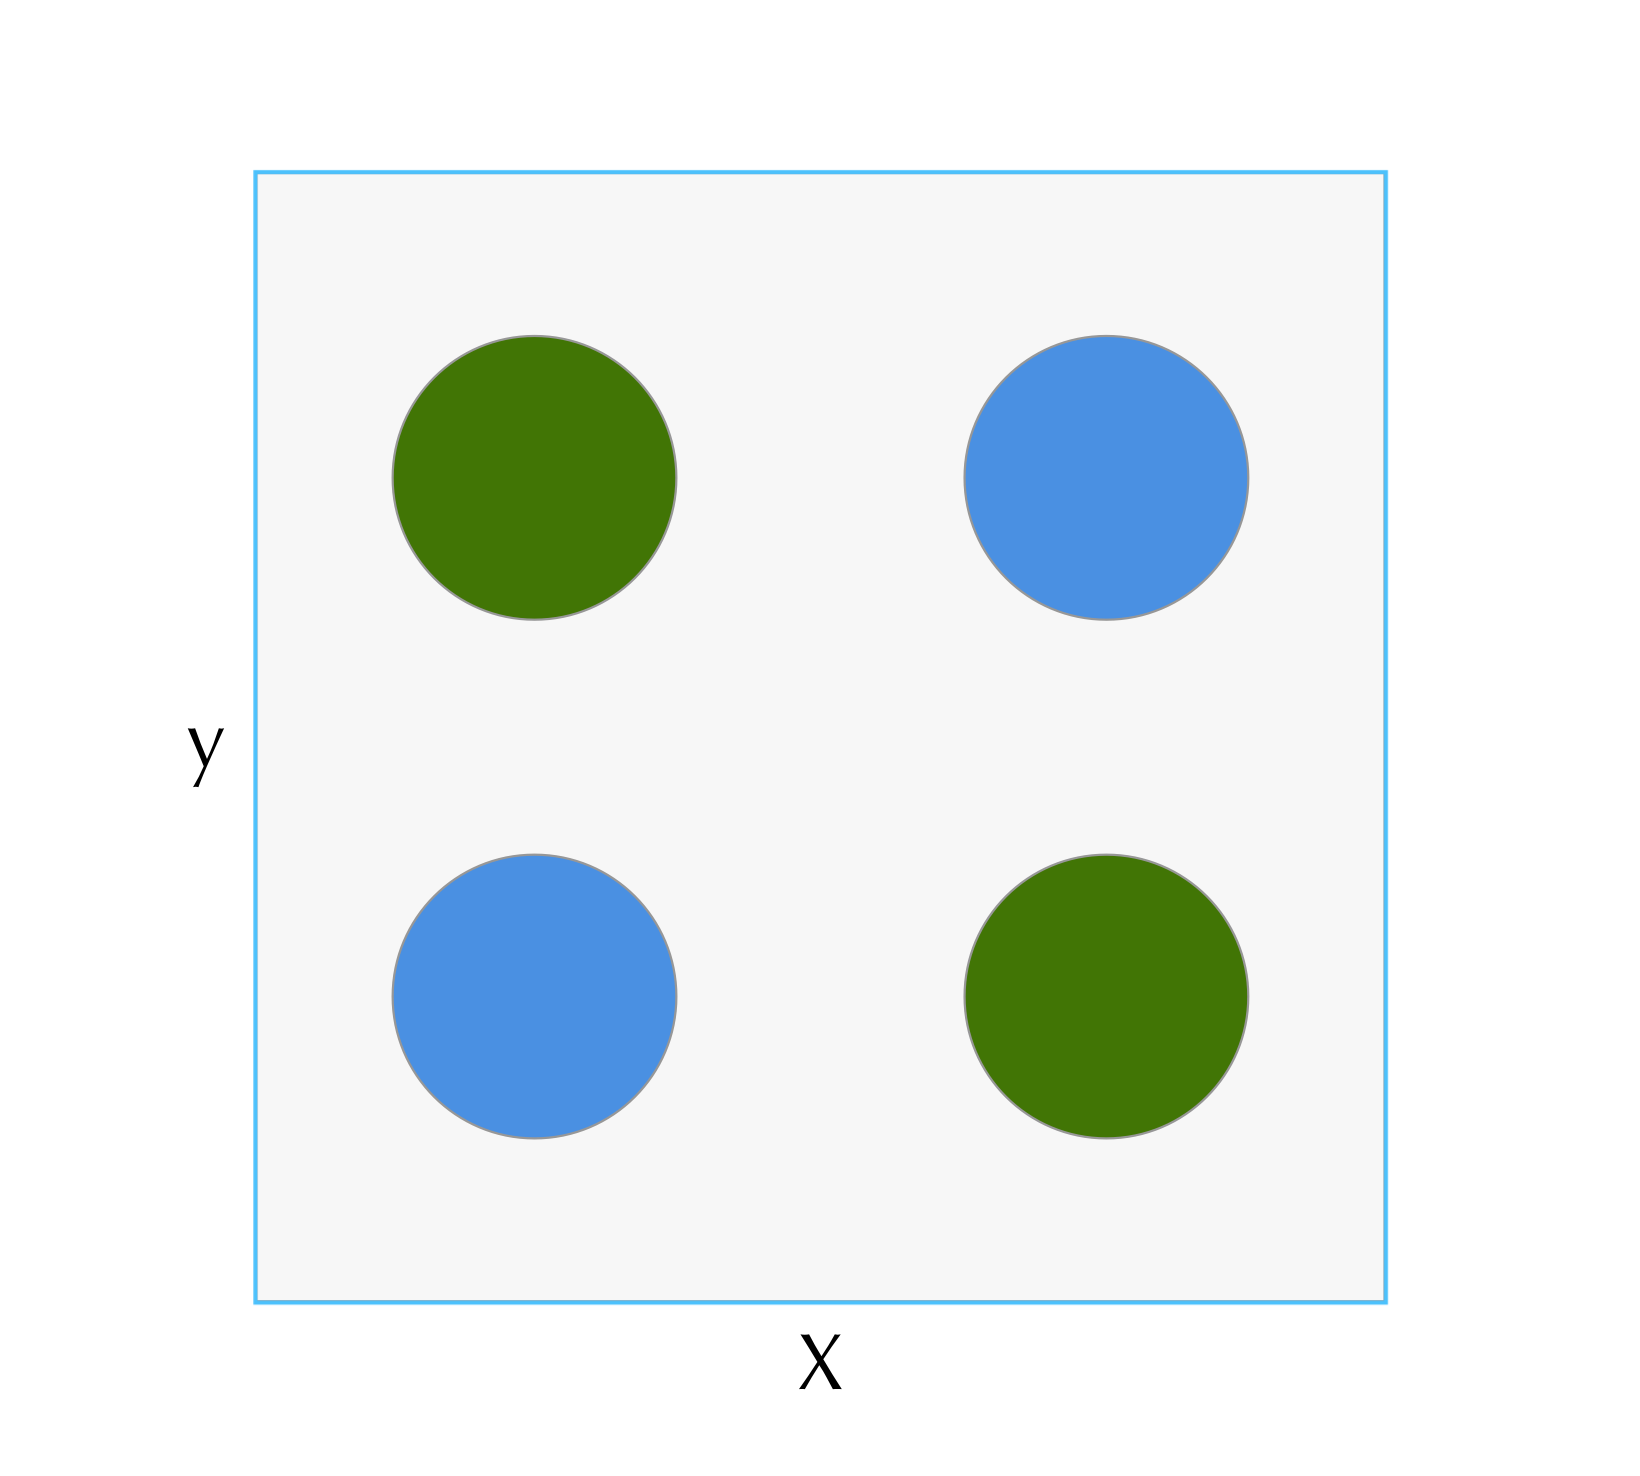
\includegraphics[width=0.5\linewidth]{figures/xor_problem} 

}

\caption{Example of the XOR problem. Classes encoded by color are not linearly seperable.}\label{fig:xorproble}
\end{figure}

It wasn't until 1986 that a realistic technique for training these
multi-layer perceptrons was introduced (\citet{backprop_1986}). Finally
all of the algorithmic pieces were in place for deep neural networks,
but interest stagnated due to the computational expense of training the
networks, a lack of data, and the success of other competing machine
learning algorithms.

Interest in the field of deep learning has had a massive resurgence in
the second decade of the 21st century. Driven by growing stores of data
and innovations in neural network architectures. One commonly cited
tipping point for the current ``deep learning revolution'' was the 2012
paper (\citet{imagenet_2012}) in which a deep convolutional neural
network won the ImageNet prize and showed massive improvements over
traditional methods.

\subsection{Biological Inspirations}\label{biological-inspirations}

The word `neural' in the `neural network' is reference to the fact that
these models derive inspiration from how the brain works. With the
individual nodes in a hidden `layer' frequently being called a `neuron'.
While the broad concepts may be similar between the way animal brains
and neural networks work, it is important to note that the similarities
end approximately at the network-ness of both systems. There has
however, been some more recent work on trying to more closely mimic the
brain structure with architectures such as capsule networks
(\citet{capsnet}). In addition, neuroscience experiments have
demonstrated that at least part of our visual system does truly perform
these hierarchical stacks of features when recognizing objects
(\citet{cnn_animals}).

\subsection{Geometric Interpretation}\label{geometric-interpretation}

Another way of thinking of how neural networks work is as a building up
a series of successive transformations of the data-space that attempt to
eventually let the data be linearly separable
((\ref{fig:geometricinterp}). In this interpretation each layer can be
seen as a shift and rotation of the data (the linear transformation),
followed by a warping of the new space (the activation function). In his
excellent blog post:
\href{http://colah.github.io/posts/2014-03-NN-Manifolds-Topology/}{Neural
Networks, Manifolds, and Topology}, Chris Olah gives an excellent visual
demonstration of this.

\begin{figure}

{\centering 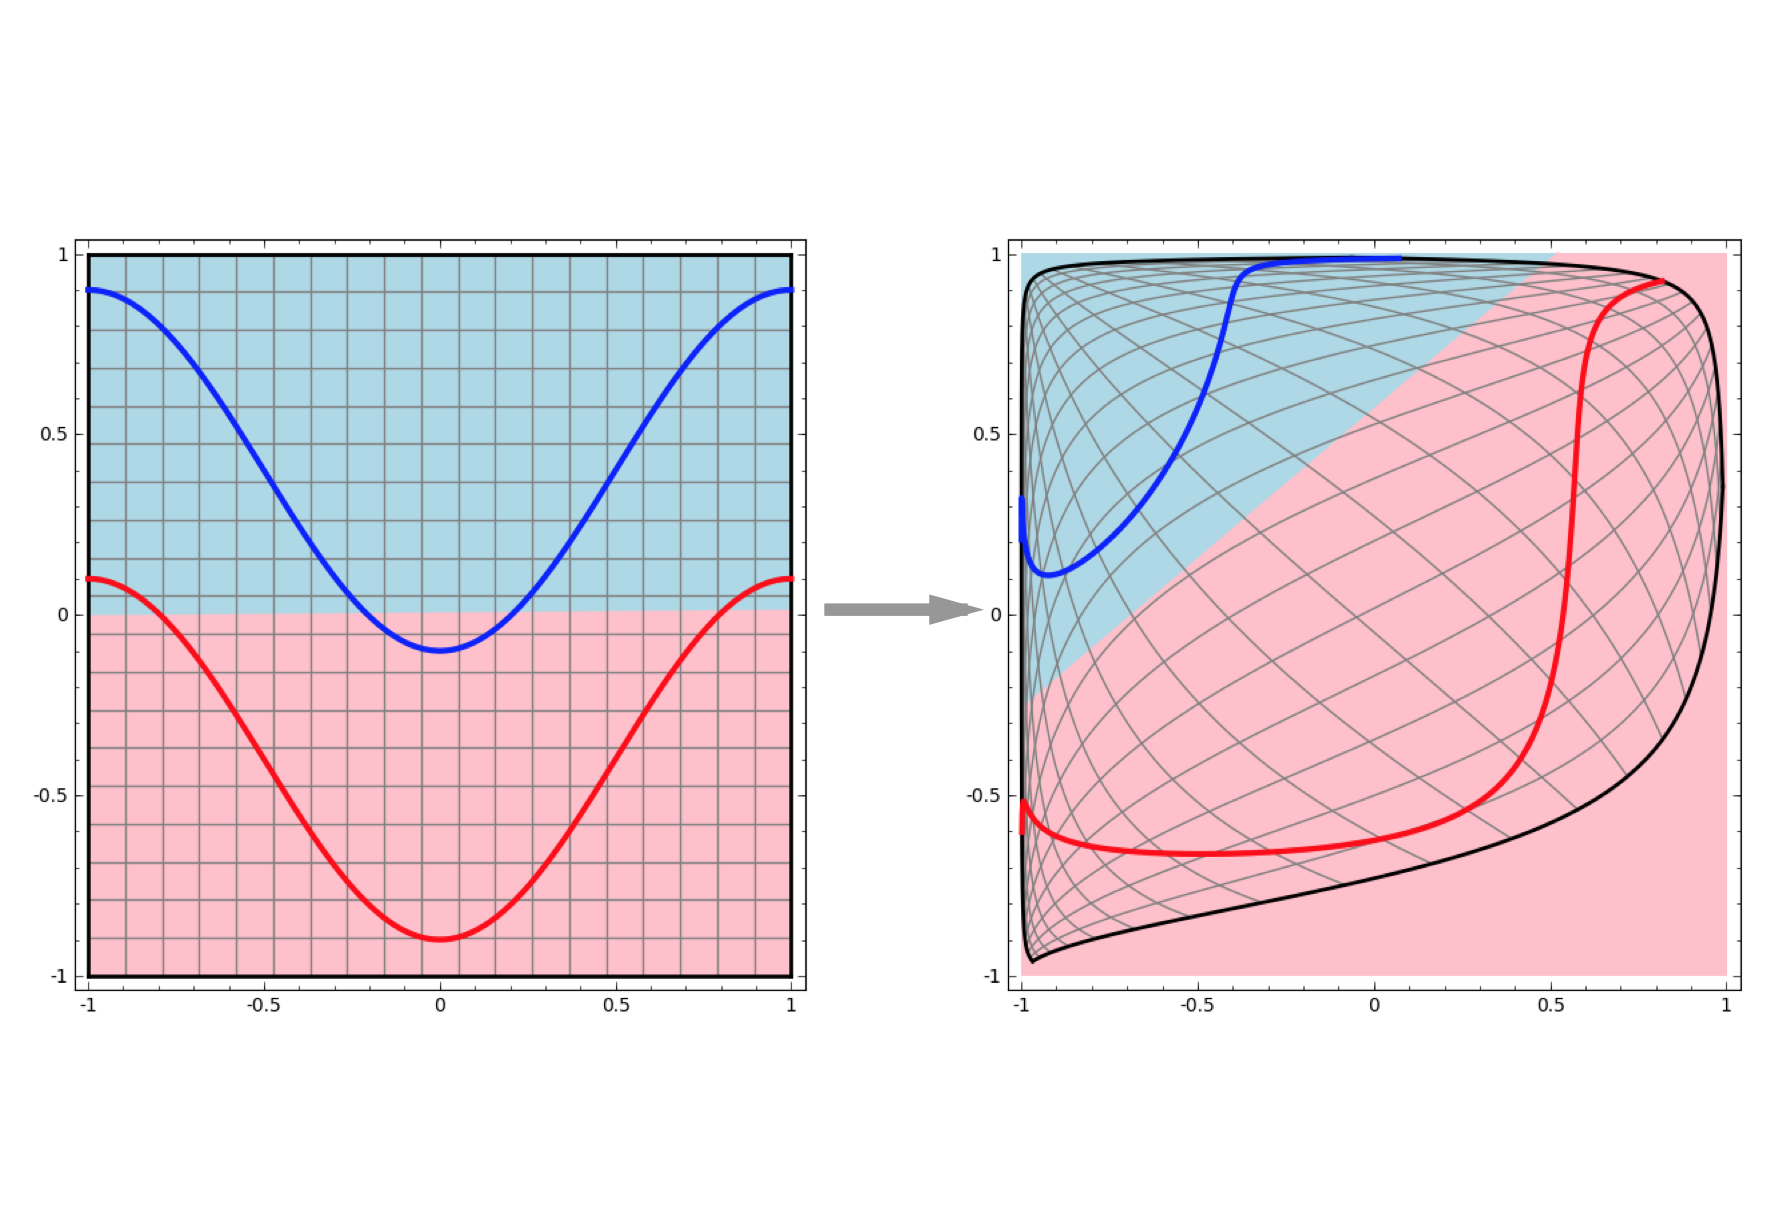
\includegraphics{figures/warp_space} 

}

\caption{Example of how a neural network can, through a series of affine transformations followed by non-linear squashings, turn a linearly inseperable proble into a linearly seperable one. Image courtesy of [Chris Olah's blog](http://colah.github.io/posts/2014-03-NN-Manifolds-Topology/)}\label{fig:geometricinterp}
\end{figure}

\section{Universal Approximation
Theorem}\label{universal-approximation-theorem}

One powerful theoretical result from neural networks is that they are
universal approximators (\citet{universal_approximators}). A neural
network with a single hidden layer and non-linear activations functions
on that layer can represent \emph{any} borel-measurable function. This
result means that there are no theoretical limits on the capabilities of
neural networks. Obviously, in real-world situations this is not the
case. We can not have infinite width hidden layers, infinite parameters
requires infinite data, and even more limiting are our inefficient
learning methods. All constraints considered though, the universal
approximation theorem does provide confidence that, as long as they are
properly constructed and trained, neural networks are amazingly flexible
models.

\section{The Computation Graph}\label{the-computation-graph}

While the building blocks of neural networks are simple, often complete
models are composed of hundreds to even thousands of neurons and
millions of connections and representing them in mathematical notation
becomes exceedingly difficult. A method of dealing with this complexity,
along with also helping in the intuition of many other properties, is to
represent the networks as a `computation graph.'

A computation graph is simply directed acyclic diagram that shows the
flow of data through the model. Each neuron is usually represented as a
circle with the weights both in and out of the neuron's value
represented as edges.

Sometimes, when the models get even larger, the layers (or groups of
neurons) will get lumped into a single node in the graph (as on the
right of the figure.)

\section{Terminology}\label{terminology}

When covering the basic mathematical operations of a neural network it
helps to have a reference for some of the terms that get used. This list
provides the most commonly used terms for the models we will be
describing.

\textbf{Neuron}: An individual node in the network. Has two values:
activation, or the value of the linear function of all inputs, and the
post-activation-function value, or a simple transformation of the
activation by the activation function.

\textbf{Affine Transformation}: A linear transformation of an input
(either data input or a hidden layer's output). Essentially a linear
regression.

\textbf{Bias Term}: A constant term added to the affine transformation
for a given neuron. Also known as an `intercept term.'. For notational
simplicity in most of our formulas we will omit this.

\textbf{Activation Function}: A non-linear function that takes an input
and `squashes' it to some range. A common activation function is the
sigmoid, which takes an unbounded real-valued input and returns a value
between -1 and 1.

\textbf{Layer}: A collection of neurons who's inputs typically share the
same inputs (either another layer's output or the data).

\textbf{Hidden Layer}: A layer who's input is the output of a previous
layer and who's output is another layer. E.g. Input layer
-\textgreater{} hidden layer -\textgreater{} output layer.

\section{Mathematical Operations}\label{mathematical-operations}

The basic operations that one does on a neural network really fall into
two categories. Forward propagation, or the passing of data into and
through subsequent layers of the model to arrive at an output, and
back-propagation, or the calculation of the gradient of each parameter
in the model by stepping back through the model from the loss function
to the input. For a more thorough treatment of these steps see
\citet{goodfellow_DL} chapter six.

\subsection{Forward Propagation}\label{forward-propagation}

Let a neural network with \(l\) layers and \(k\) dimensional input \(X\)
and \(m\) dimensional output \(\hat{y}\) attempting to predict the true
target \(y\). Each layer is composed of \(s_i, i \in \{1, 2, ...,l\}\)
neurons and has respective non-linear activation function \(f_i\). The
output of a layer after affine transformation is represented as a vector
of length \(s_i\): \(\underline{a_i}\) and the layer ouput vector
post-activation function outputs: \(\underline{o_i}\). The weights
representing the affine transition from one layer \(i\) to layer \(j\)
are a matrix \(W_i\) of of size \(s_{i} \times s_j\). Finally the
network has a differentiable with respect to \(\hat{y}\) loss function:
\(L(\hat{y}, y)\).

Forward propagation then proceeds as follows.

\begin{enumerate}
\def\labelenumi{\arabic{enumi}.}
\tightlist
\item
  Input \(X\) \((1 \times k\)) is multiplied by \(W_1\) (size
  \((k\times s_i)\) ) to achieve the \emph{activation values} of the
  first hidden layer.

  \begin{itemize}
  \tightlist
  \item
    \(X \cdot W_1 = \underline{a_1}\)
  \end{itemize}
\item
  The \((1 \times s_1)\) activation vector of the first layer is then
  run element-wise though the first layer's non-linear activation
  function to achieve the output of layer 1.

  \begin{itemize}
  \tightlist
  \item
    \(\underline{o_1} = f_1(\underline{a}_1)\)
  \end{itemize}
\item
  This series of operations is then repeated through all the layers,
  (using the subsequent layers output vector as the input to the next
  layer,) until the final layer is reached.

  \begin{itemize}
  \tightlist
  \item
    \(\underline{o_i} = f_i(\underline{o_{(i - 1)}} \cdot W_i)\)
  \end{itemize}
\item
  Finally, the loss is calculated from the output of our final layer.

  \begin{itemize}
  \tightlist
  \item
    \(L_n = L(\underline{o_l}, y) = L(\hat{y}, y)\)
  \end{itemize}
\end{enumerate}

While not strictly necessary for forward propagation, the intermediate
layer activations and output vectors are kept stored so they can be used
in the later calculation of the gradient via back propagation.

\subsection{Back Propagation}\label{back-propagation}

If we are just looking to gather predictions from our model we can stop
at forward propagation. However, most likely we want to train our model
first. The most common technique for training neural networks is using a
technique called back propagation (\citet{backprop_1986}). In this
algorithm the chain rule is used to walk back through the layers of the
model starting from the loss function to the input weights in order to
calculate each weight's gradient with respect to the loss. This gradient
is then descended using any number of gradient descent algorithms.

\subsubsection{The Chain Rule}\label{the-chain-rule}

Back propagation is nothing more than a repeated application of the
chain rule from calculus. Let \(x\) be a single dimensional real valued
input that is mapped through first equation \(f\) and then \(g\), both
of which map from a single dimensional real number to another single
dimensional real number: \(f(x) = z, g(z) = y\) or \(g(f(x)) = y\). The
chain rule states that we can calculate the derivative of the outcome
with respect to the input by a series of multiplications of the
derivatives of the composing functions.

\begin{equation} 
  \frac{dy}{dx} = \frac{dy}{dz}\frac{dz}{dx}
  \label{eq:chainrule}
\end{equation}

This single dimensional example could be thought of as a neural network
composed of two layers, each with a single dimension. The single
dimensional case is illuminating, but the value of the chain rule comes
when it is applied to higher dimensional values.

\subsubsection{Expanding to higher
dimensions}\label{expanding-to-higher-dimensions}

Now, let \(\mathbb{x} \in \mathbb{R}^m\) and
\(\mathbb{z} \in \mathbb{R}^n\). The function \(f\) maps from
\(\mathbb{R}^m \to \mathbb{R}^n\) and
\(g: \mathbb{R}^n \to \mathbb{R}\). Further, let
\(\textbf{z} = f(\textbf{x})\) and \(y = g(\textbf{z})\). The chain rule
can then be expressed as:

\begin{equation} 
  \frac{dy}{dx_i} = \sum_{j}\frac{dy}{dz_j}\frac{dz_j}{dx_i}
  \label{eq:chainrulemv}
\end{equation}

Or that the derivative of \(y\) with respect to the \(i^{\text{th}}\)
element of \(\textbf{x}\) is the sum of the series of products of the
derivatives of result \(\textbf{z}\) that sits between the two values in
the function composition.

Another way of thinking of this is, the derivative of the output of the
function composition \(f \circ g\) with respect to some element of the
input is the sum of all of the derivatives of all of the paths leading
from the input element to the output.

\begin{figure}

{\centering 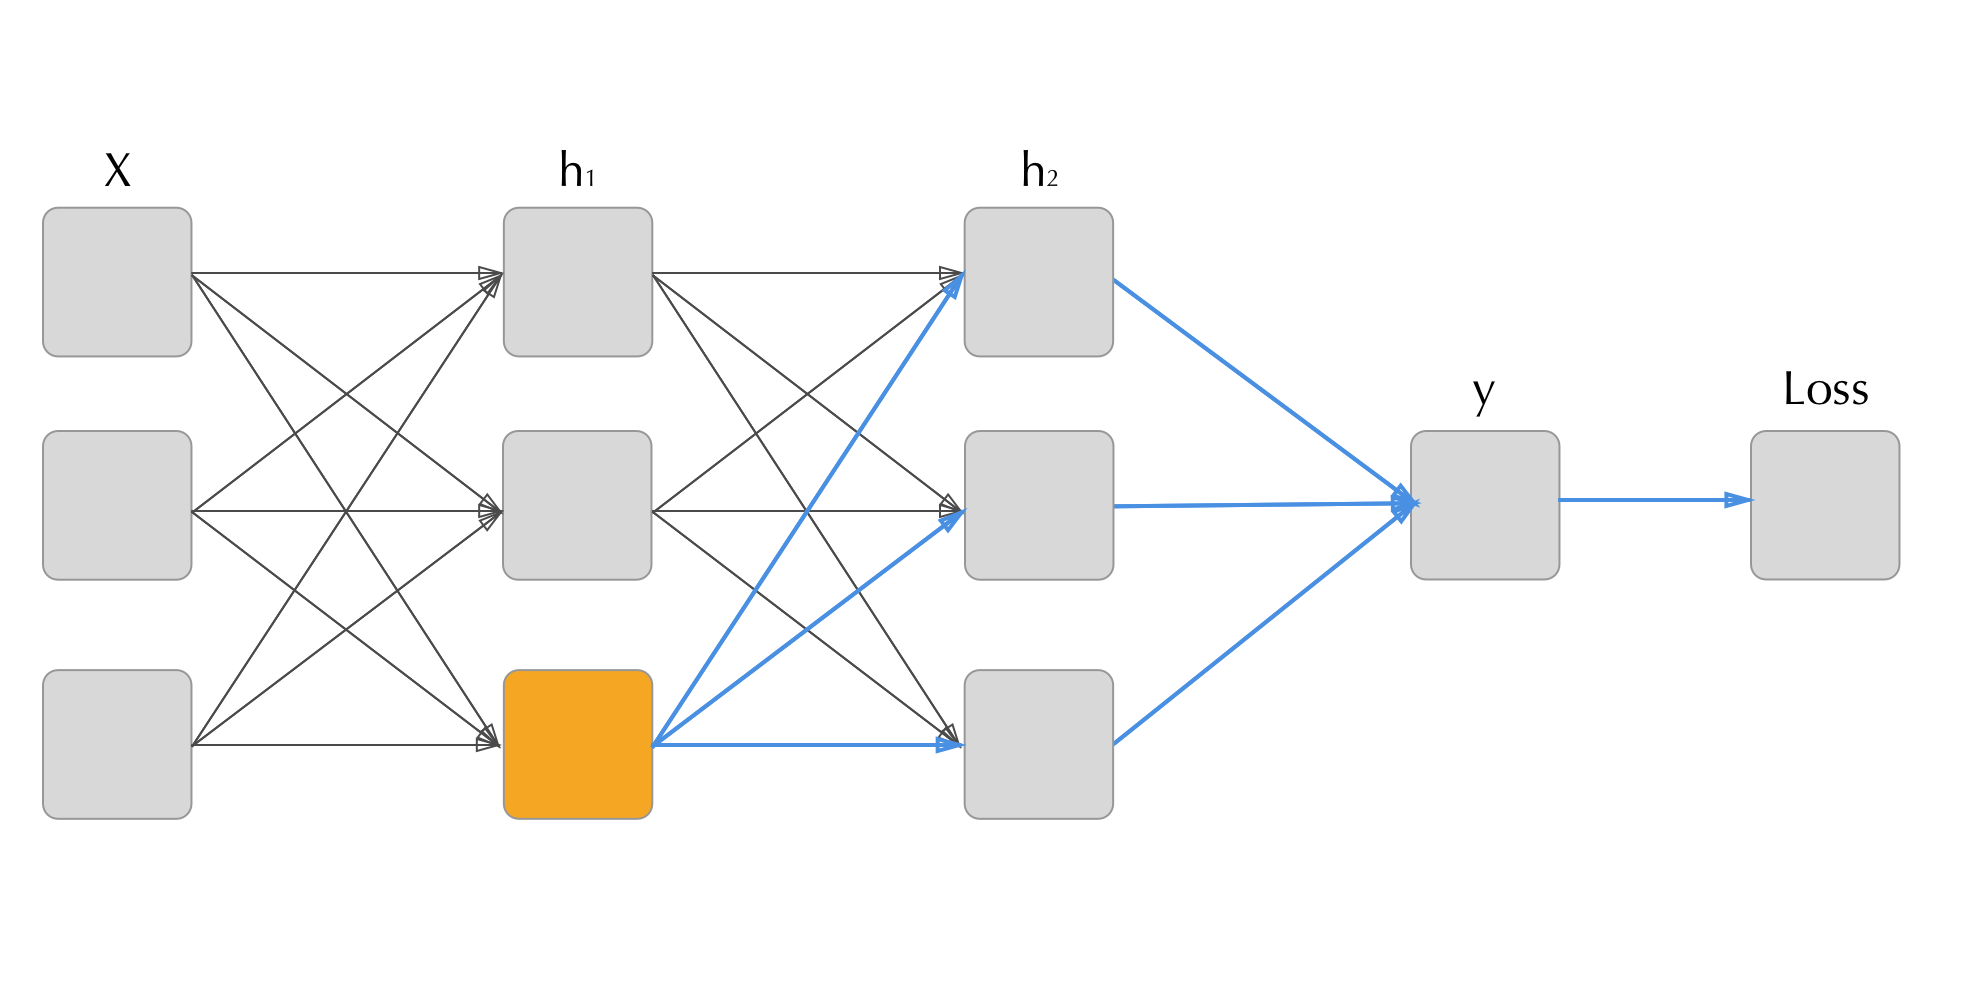
\includegraphics{figures/backprop} 

}

\caption{How back Propagation steps back from the output to the input. To calculate the gradient with respect to the loss of the orange neuron the we need to aggregate the gradients of all connected points further along in the computation graph (blue connections).}\label{fig:unnamed-chunk-1}
\end{figure}

\subsubsection{Applied to Neural
Networks}\label{applied-to-neural-networks}

To apply this technique to neural networks we need to make sure all
components of our network are differentiable and then walk back from the
loss function to the last (or output) layer, calculating the gradients
of the output layer's neurons with respect to the loss. Once we have
calculated the gradients with respect to the weights of the output layer
we only need use those calculated gradients to calculate the gradients
of the preceding layer. We can then proceed layer by layer, walking back
through the model filling out each neuron's weight gradients until we
reach the input.

To calculate the gradient of the weights for hidden layer \(i\) we can
recall that the hidden layers output can be represented as
\(\textbf{a}_i = f_i(\textbf{W}\cdot\textbf{a}_{(i -1)})\) (we're
omitting the bias term here for simplicity). Thus to calculate the
gradient's on the weights we can set
\(\textbf{g}^*_i = \textbf{g}_{i+1} \odot f'(a_{i+1})\) to be the
gradient un-activated by our layer's activation function's derivative.
Then to find the derivative with respect to each neuron's weights within
the layer we multiply this un-activated gradient by the transpose of the
layer's output vector: \(\textbf{g}_i = \textbf{g}^*_i \textbf{o}_i^t\).

The fact that the calculation of these gradients is so simple is
fundamental to deep learning. If it were more complicated, extremely
large networks (such as those used in computer vision) with millions of
parameters to tune would simply be computationally infeasible to
calculate gradients for. Conveniently, the run time of the back
propigation is a simple product of the number of neurons in each layer
and the number of layers in the whole model.

\subsubsection{Other methods}\label{other-methods}

Non-gradient based techniques have been explored for neural networks but
have ultimately proven to slow for any realistic sized network. For
instance evolutionary strategies (\citet{evostrat}), a new technique
proposed by a group at OpenAi uses random searches of the parameter
space with evolutionary algorithms to tune the model's parameters.
However, since often these parameter spaces are millions of dimensions,
an extremely large number of random perturbations are needed to inform a
good direction to move{[}\^{}These do find use when methods are used
when the loss function does not have a gradient. Such as reinforcement
learning scenarios.{]}.

\section{Training}\label{training}

\subsection{Gradient Descent}\label{gradient-descent}

Once the gradient is computed, optimization proceeds the same way any
gradient-based optimization problem does. The simplest algorithm for
doing so being the steepest descent algorithm. In this algorithm, each
weight for our network is updated by adding its gradient multiplied by a
small scalar called a `learning rate' (\(\alpha\)).

\[\theta^{(j)} = \theta^{(j - 1)} + \alpha\Delta_{\theta}\]

The new updated weights are then used in another forward propagation,
followed by another back propagation and weight update. This processes
is repeated until the loss finds a minimum or some other stopping
criteria is defined (such as a given number steps) is satisfied.

\subsection{Gradient Descent
Modifications}\label{gradient-descent-modifications}

There are many scenarios in which traditional steepest descent is not an
ideal for finding minimums of the loss function. A classic example is
when the loss function takes the form of a long trough
(\ref{fig:badloss}. In this case steepest descent will spend most of its
time bouncing around between the sides of the trough due to over
stepping the low point, thus wasting many of its iterations undoing its
previous work rather than progressing in the true direction of the
minimum.

\begin{figure}

{\centering \includegraphics[width=0.6\linewidth]{http://www.nbertagnolli.com/assets/descent_methods/GDWBLS} 

}

\caption{Demonstration of steepest descents limitations on trough like gradient surfaces. Much of each step's progress is wasted on bouncing back and forth between the two walls of the gradient rather than descending directly towards the minimum. Image from [Nicolas Bertagnolli's blog](http://www.nbertagnolli.com/)}\label{fig:badloss}
\end{figure}

One of the most common additions to plain gradient descent is the
addition of momentum. Momentum makes each step a function of not only
the current gradient but also a decaying average of previous
generations. For a thorough overview of momentum based methods see
\citet{momentum}.

\section{Activation Functions}\label{activation-functions}

There are many different possible activation functions. The only
conditions that an activation function needs to satisfy is that it takes
an unbounded real input and returns some non-linear transformation of
that input that is differentiable with respect to the input.

One of the simplest functions used is the sigmoid which simply squashes
the neuron's activation from all real numbers to between 0 and 1. A
newer and extremely common choice is the rectified linear unit (Relu)
function (\citet{relu_paper}).

\BeginKnitrBlock{definition}[sigmoid activation function]
\protect\hypertarget{def:sigmoid}{}{\label{def:sigmoid} \iffalse (sigmoid
activation function) \fi{} }\[f(x) = e(x)/(1 + e(x))\]
\EndKnitrBlock{definition}

\BeginKnitrBlock{definition}[Rectified Linear Unit activation function]
\protect\hypertarget{def:relu}{}{\label{def:relu} \iffalse (Rectified Linear
Unit activation function) \fi{} }\[f(x) = \text{max}(0,x)\]
\EndKnitrBlock{definition}

\begin{verbatim}
## Warning in .doLoadActions(where, attach): trying to execute load actions
## without 'methods' package
\end{verbatim}

\begin{verbatim}
## Warning: replacing previous import by 'tidyr::%>%' when loading 'broom'
\end{verbatim}

\begin{verbatim}
## Warning: replacing previous import by 'tidyr::gather' when loading 'broom'
\end{verbatim}

\begin{verbatim}
## Warning: replacing previous import by 'tidyr::spread' when loading 'broom'
\end{verbatim}

\begin{verbatim}
## -- Attaching packages ------------------------------------------------------------------------- tidyverse 1.2.1 --
\end{verbatim}

\begin{verbatim}
## √ ggplot2 2.2.1     √ purrr   0.2.4
## √ tibble  1.3.4     √ dplyr   0.7.4
## √ tidyr   0.7.2     √ stringr 1.2.0
## √ readr   1.1.1     √ forcats 0.2.0
\end{verbatim}

\begin{verbatim}
## -- Conflicts ---------------------------------------------------------------------------- tidyverse_conflicts() --
## x dplyr::filter() masks stats::filter()
## x dplyr::lag()    masks stats::lag()
\end{verbatim}

\begin{figure}

{\centering 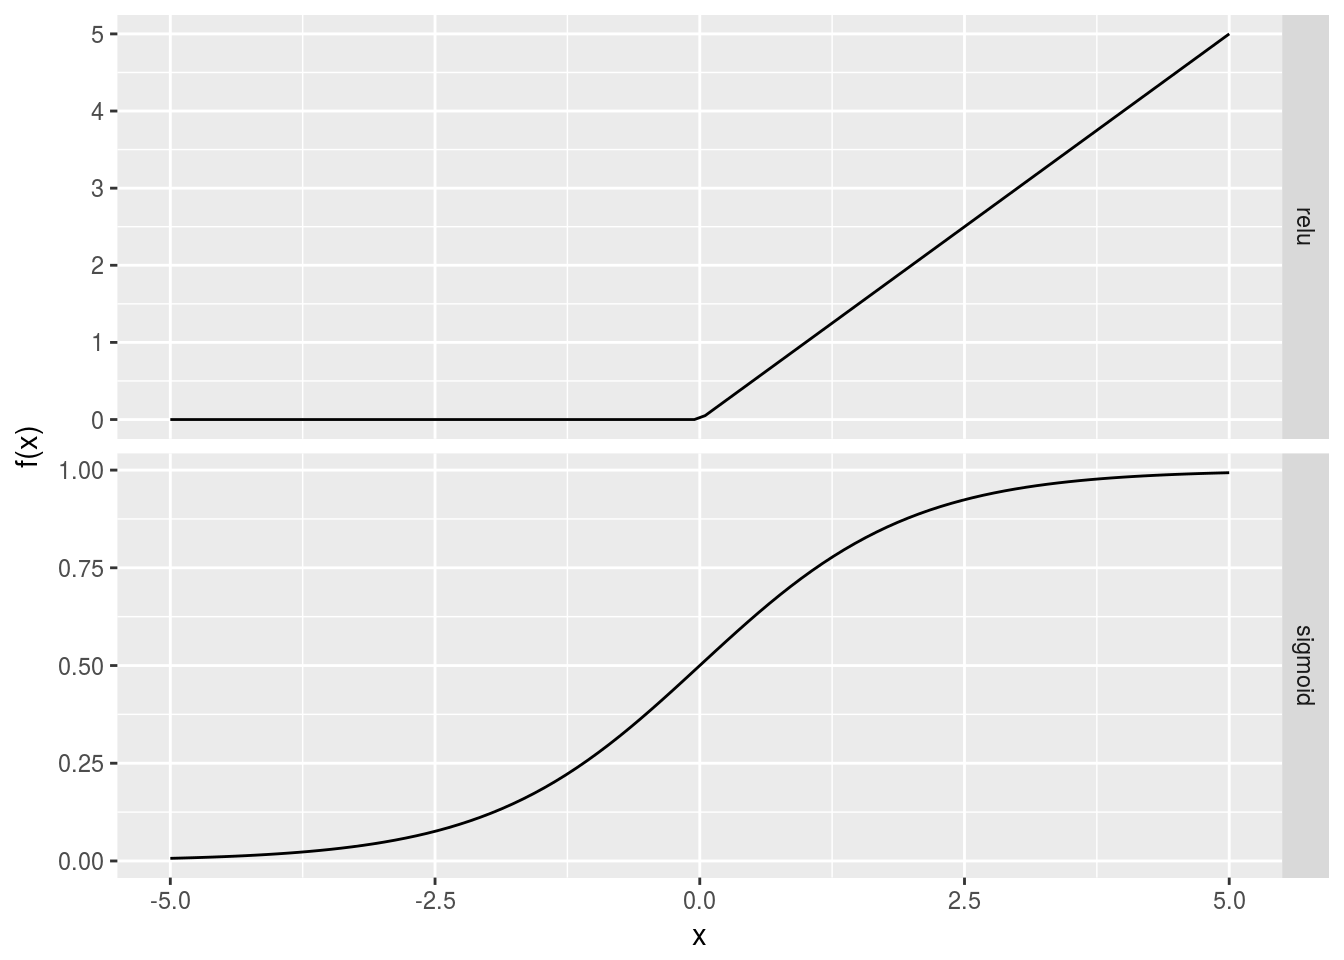
\includegraphics[width=0.85\linewidth]{bookdown-demo_files/figure-latex/unnamed-chunk-2-1} 

}

\caption{Comparison of the relu and sigmoid activation functions.}\label{fig:unnamed-chunk-2}
\end{figure}

Another, popular loss function that is used on the output layer when
predicting categories is the softmax function. Unlike the previously
mentioned loss functions this one takes a vector \(\textbf{o}\) of
length \(m\) representing the output of each of the layer's neurons.

\BeginKnitrBlock{definition}[Softmax activation function.]
\protect\hypertarget{def:softmax}{}{\label{def:softmax} \iffalse (Softmax
activation function.) \fi{}
}\[f(\textbf{o})_i = \frac{\text{exp}(o_i)}{\sum_{j = 1}^m \text{exp}(o_j)}\]
\EndKnitrBlock{definition}

This function serves to turn the output of a layer into a multivariate
probability vector. The \(m\) outputs of the softmax sum to one.
\footnote{It is important to note that, while the values sum to one,
  it's not a true probability output, but will help indicate which class
  is most likely and roughly by what magnitude over other potential
  class choices.}

\section{Loss functions}\label{loss-functions}

Like any machine learning model, neural networks have a loss function
(sometimes called a cost function), or a function that helps the model
know how close it is to performing as desired. As previously mentioned,
in the case of neural networks we almost always want our loss function
to be differentiable with respect to our model's output
\(\hat{\textbf{y}}\) as the derivative is needed for calculating the
gradient on which the model is trained.

Almost always the loss function is derived from the model's likelihood
and serves as a maximum likelihood estimator.

If we let \(\theta\) represent the parameters (weights) of our model
with input \(\textbf{x}\) and output \(\textbf{y}\). The negative
log-likelihood of our model is minimized when the Kullback Leibler
divergence between our estimated model and the truth is minimized. Thus
we can view training as traversing the space of \(\theta\) in an attempt
to find values that return the lowest value to this function.

\BeginKnitrBlock{definition}[General maximum likelihood loss function]
\protect\hypertarget{def:negloglik}{}{\label{def:negloglik}
\iffalse (General maximum likelihood loss function) \fi{}
}\[J(\theta) = - \mathbb{E}_{x,y \sim \hat{p} \text{ data}} \log{{p_{\text{model}}(\textbf{y} |\textbf{x} })}\]
\EndKnitrBlock{definition}

Of course, the precise form of the maximum likelihood loss function will
change depending on the model. Next we will briefly introduce the two
classes of loss functions: regression and classification, and the most
commonly used functions within those classes.

\subsection{Regression loss functions}\label{regression-loss-functions}

When fitting a neural network who's outcome is a single real numbered
variable \(\hat{y}\) the most common loss function used is the mean
square error.

\BeginKnitrBlock{definition}[Mean squared error loss]
\protect\hypertarget{def:mse}{}{\label{def:mse} \iffalse (Mean squared error
loss) \fi{}
}\[\text{MSE}(\theta) = -\frac{1}{n} \sum_{i = 1}^{n} (\hat{y}^{(i)} - y^{(i)})^2\]

Where \(y_i\) represents the outcome of the \(i^{\text{th}}\)
observation of \(n\) training observations.
\EndKnitrBlock{definition}

This assumes that the output, when conditioned on the input, takes the
form of a normal distribution. Minimizing the mean squared error is
equivalent to maximizing the conditional normal likelihood function
(\citet{goodfellow_DL} chapter 5.5) and is thus a maximum likelihood
method.

\subsection{Classification loss
functions}\label{classification-loss-functions}

There are two separate instances of classification that need to be
considered. The binary case, where we are classifying a yes or no answer
for a single class, or a categorical case, where we have more than two
possible classes to choose from and need to place our data into one of
them.

In the single outcome case the approach is to assume the outcome is a
Bernoulli distribution over outcome \(y\) conditioned on the input
\(x\). The resultant loss function is commonly referred to as `binary
cross entropy.'\footnote{It is interesting to note that while we
  typically only use the term `cross entropy' for categorical outcomes,
  any time we are minimizing KL or maximizing the likelihood we are
  minimizing the cross entropy. So technically we could also call the
  mean squared error the `continuous cross entropy loss.'}

\BeginKnitrBlock{definition}[Binary cross entropy loss]
\protect\hypertarget{def:crossentropy}{}{\label{def:crossentropy}
\iffalse (Binary cross entropy loss) \fi{}
}\[L(\theta) = -\frac{1}{n}\sum_{i = 1}^n\left[ y_i\log(\hat{y}_i) + (1 - y_i)\log(1 - \hat{y}_i)\right]\]
\EndKnitrBlock{definition}

This can be generalized into the multivariate case by swapping a
multinomial model as the conditional distribution and thus adding more
terms to the internal summation representing each possible class and its
assigned probability.

\BeginKnitrBlock{definition}[Categorical cross entropy loss]
\protect\hypertarget{def:catcrossentropy}{}{\label{def:catcrossentropy}
\iffalse (Categorical cross entropy loss) \fi{}
}\[L(\theta) = -\frac{1}{n}\sum_{i = 1}^n\sum_{j = 1}^k y_{i,j}\log(\hat{y}_{i,j})\]

Where \(y_{i,j}\) represents the \(i^{\text{th}}\) observation's value
for the \(k^{\text{th}}\) category (dummy encoded).
\EndKnitrBlock{definition}

\subsection{Other loss functions}\label{other-loss-functions}

While it is possible to use other loss functions in neural networks, it
is commonly not advised as the maximum-likelihood methods perform just
as well and usually results in a more robust fit to the data. As deep
learning situations usually have a large number of training observations
the Cramer-Rao lower bound property, that a maximum likelihood estimator
has the lowest variance of any consistent estimator, is particularly
relevant. For a more thorough overview of the common loss functions used
in deep learning see \citet{goodfellow_DL} chapter six.

\chapter{Architectures For Sequence Learning}\label{architectures}

In the previous chapter we described the general neural network
architecture. This is usually called a dense feed-forward network.
`Dense' refers to the fact that all neurons of a given layer are
connected to all neurons of the successive layer. `Feed-forward' refers
to the fact that data flows into the network and straight to the output,
traveling only forward through the layers. In this section we will
expand upon this general model with different architectures: the
recurrent neural network (RNN) (\citet{rnn_intro}) and the convolutional
neural net (CNN) (\citet{cnn_intro}).

While they are often represented as very different models, these
architectures are in fact sub-models of the dense feed-forward networks
from the last chapter, just with restrictions placed on weights in the
form of deleting connections (setting weight to 0) or sharing weights
between multiple connections.

These restrictions applied to standard neural networks allow the models
to more efficiently model tasks related to sequential data by reducing
the number of parameters that need to be fit or, in some cases, helping
with the propagation of the gradients for efficient training.

\section{Terminology}\label{terminology-1}

Throughout this chapter we will refer to an input \(\mathbf{x}\) which
is a vector of observations at \(t\) time points. In addition, we have
an outcome \(\mathbf{y}\), also of length \(t\) that represents some
state or property of the system generating \(x\) at each time point.
This could be the type of road a car is driving on, the sentiment of a
speaker, or the next \(x_i\) value (e.g.~next word in a sentence).

\section{Recurrent Neural Networks}\label{recurrent-neural-networks}

One way to efficiently deal with the fact that sequential data is often
highly correlated between observations is to fit a model to each
time-point and then pass it information on what was happening prior. The
model can then combine the previous information with the newly observed
input to come up with a prediction.

This can be accomplished in a neural network by adding recurrent links
between layers. Typically, this is done by passing the hidden layer (or
layers) of the network the values of itself at the previous time point.
I.e. \(\mathbf{h}_{t} = g(\mathbf{x}_t, \mathbf{h}_{t - 1})\). The idea
behind this is that the hidden layer learns to encode some `latent
state'\footnote{This is in contrast with hidden markov models, which
  force the state use to infer the next step to be of the possible
  classes.} of the system that is informative for its output, and so
letting the model know what that latent state was previously will help
it update the latent state and provide an accurate output.

Why not just pass the output at time \((t-1)\) to the hidden state at
\(t\) instead? While this is possible, and indeed works much better than
not communicating information between time points at all, it suffers
from the squashing of the latent state information to out outcome of
interest. This results in a loss of information about what is happening
in the system since the hidden or latent state to the outcome is not
necessarily a one-to-one function. In addition, there is convenience in
the fact that the hidden state is already of the same dimension,
allowing for a simple element-wise addition of the components from the
previous hidden state and the new input information.

\begin{figure}

{\centering 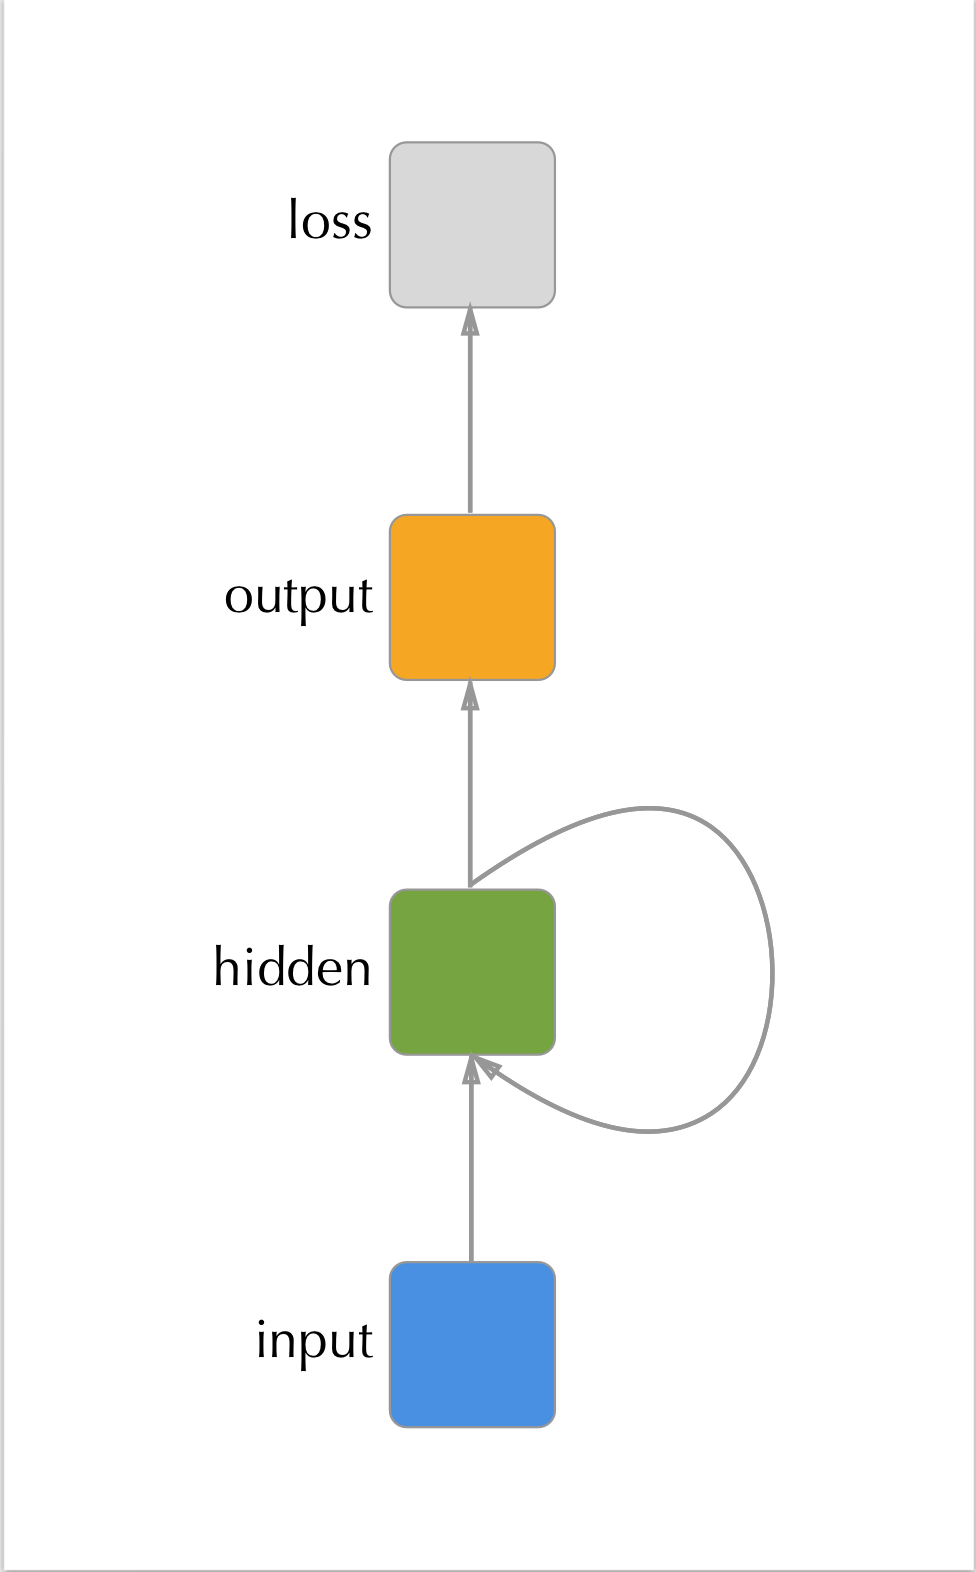
\includegraphics[width=0.4\linewidth]{figures/rnn_compact} 

}

\caption{A recurrent neural network with a single hidden layer. The hidden layer's values at time $t$ are passed to the hidden layer at time $(t + 1)$.}\label{fig:cyclegraph}
\end{figure}

\subsection{Applications to sequential
data}\label{applications-to-sequential-data}

RNNs are fundamentally models for performing analysis on sequential data
(although they have been applied to static inputs and used to generate
sequential outputs (\citet{rnn_captions})). Some of the major success
stories in recurrent neural networks come in the realm of machine
translation. For instance, Google's entire translation service is now
powered by RNNs (\citet{google_translate}).

Other domains in which RNNs have been successfully applied is in
time-series regression (\citet{rnn_regression}), speech recognition
(\citet{rnn_speach}), and handwriting recognition
(\citet{rnn_handwriting}).

\begin{figure}

{\centering 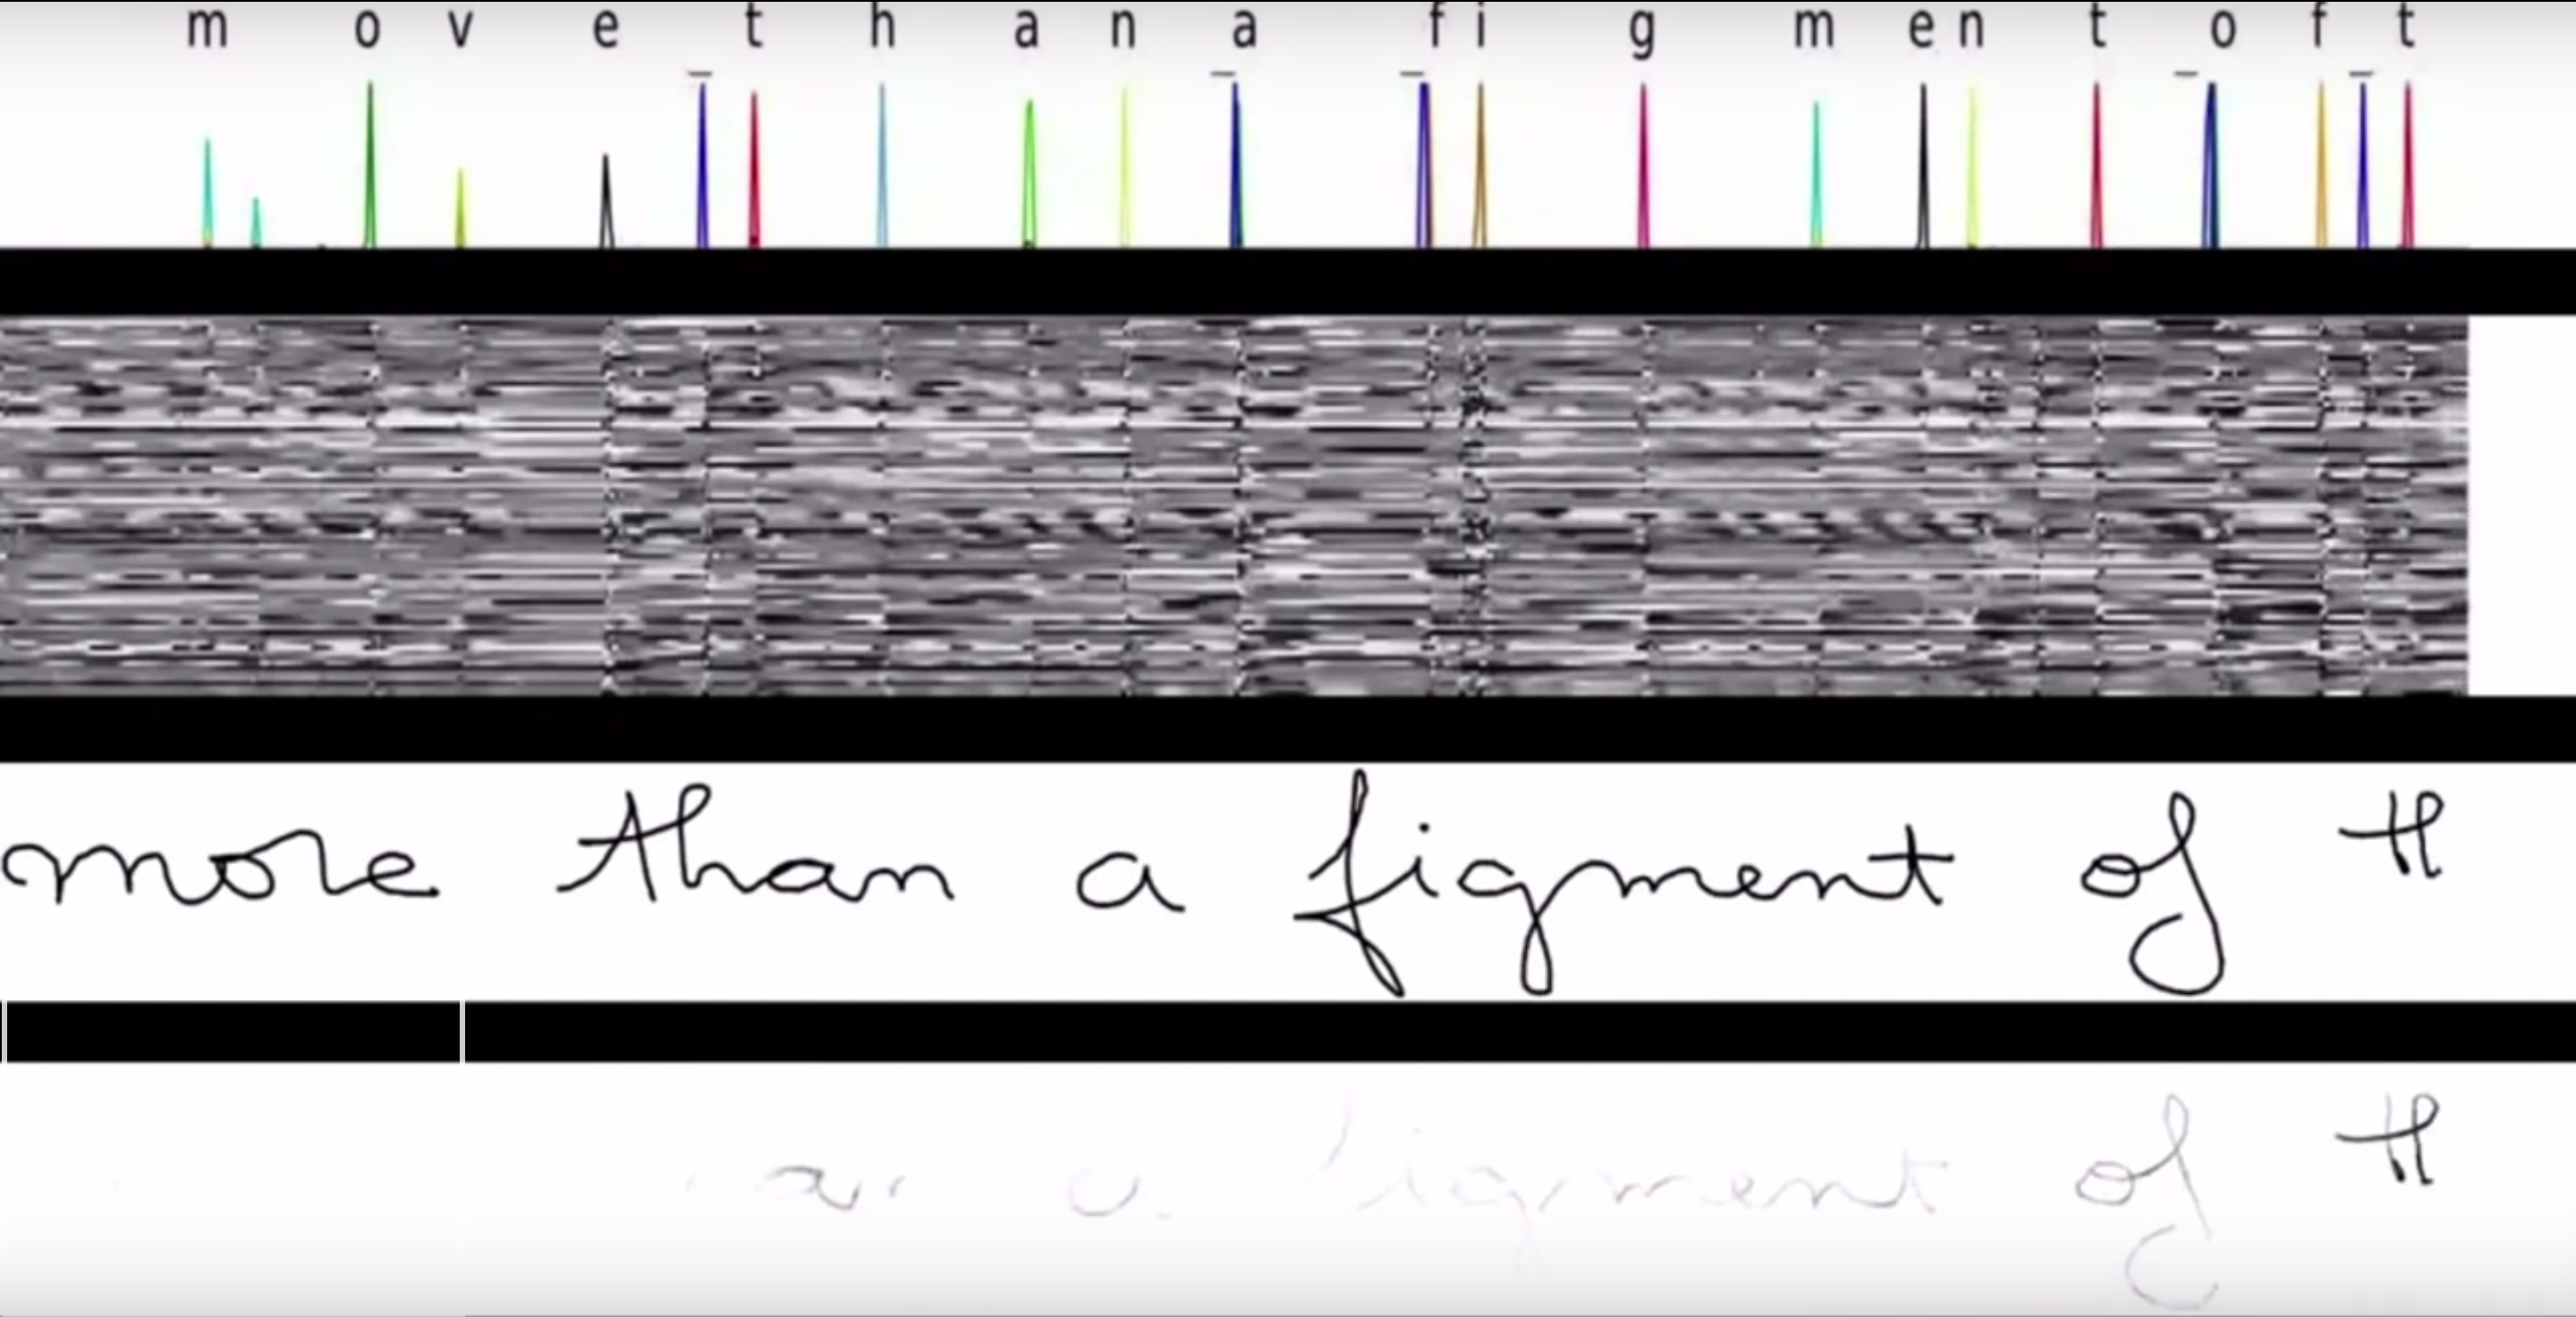
\includegraphics[width=0.9\linewidth]{figures/handwriting_rnn} 

}

\caption{Example of an RNN's output for recognizing characters in handwritten characters. The model scans along one slice at a time of the data and the output is character likelihood. Still from [youtube video](https://www.youtube.com/watch?v=mLxsbWAYIpw) by Nikhil Buduma.}\label{fig:unnamed-chunk-3}
\end{figure}

\subsection{Successes in natural language
processing}\label{successes-in-natural-language-processing}

One of the areas that has seen great results from the application of
RNNs is natural language processing. Natural language processing (or
NLP) refers broadly to the modeling of textual data in order to infer
things like sentiment, predict next words, or even generate entirely new
sentences.

Usage of neural networks for these tasks has greatly improved upon
previous techniques that constrained were constrained by linear
assumptions (e.g.~word2vec (\citet{word2vec})) or limited ability to
look backwards in time.

\subsection{Cyclical Computation
Graph}\label{cyclical-computation-graph}

A natural question that arises from the cyclical computational graph
shown in figure \ref{fig:cyclegraph} is how the gradient can be
calculated via back propagation. In fact, the cycle as represented is
just a visual simplification of the true computational graph. The
`unrolled' graph can be thought of as a long chain of neural networks
that share connections between sequential hidden layers.

\begin{figure}

{\centering 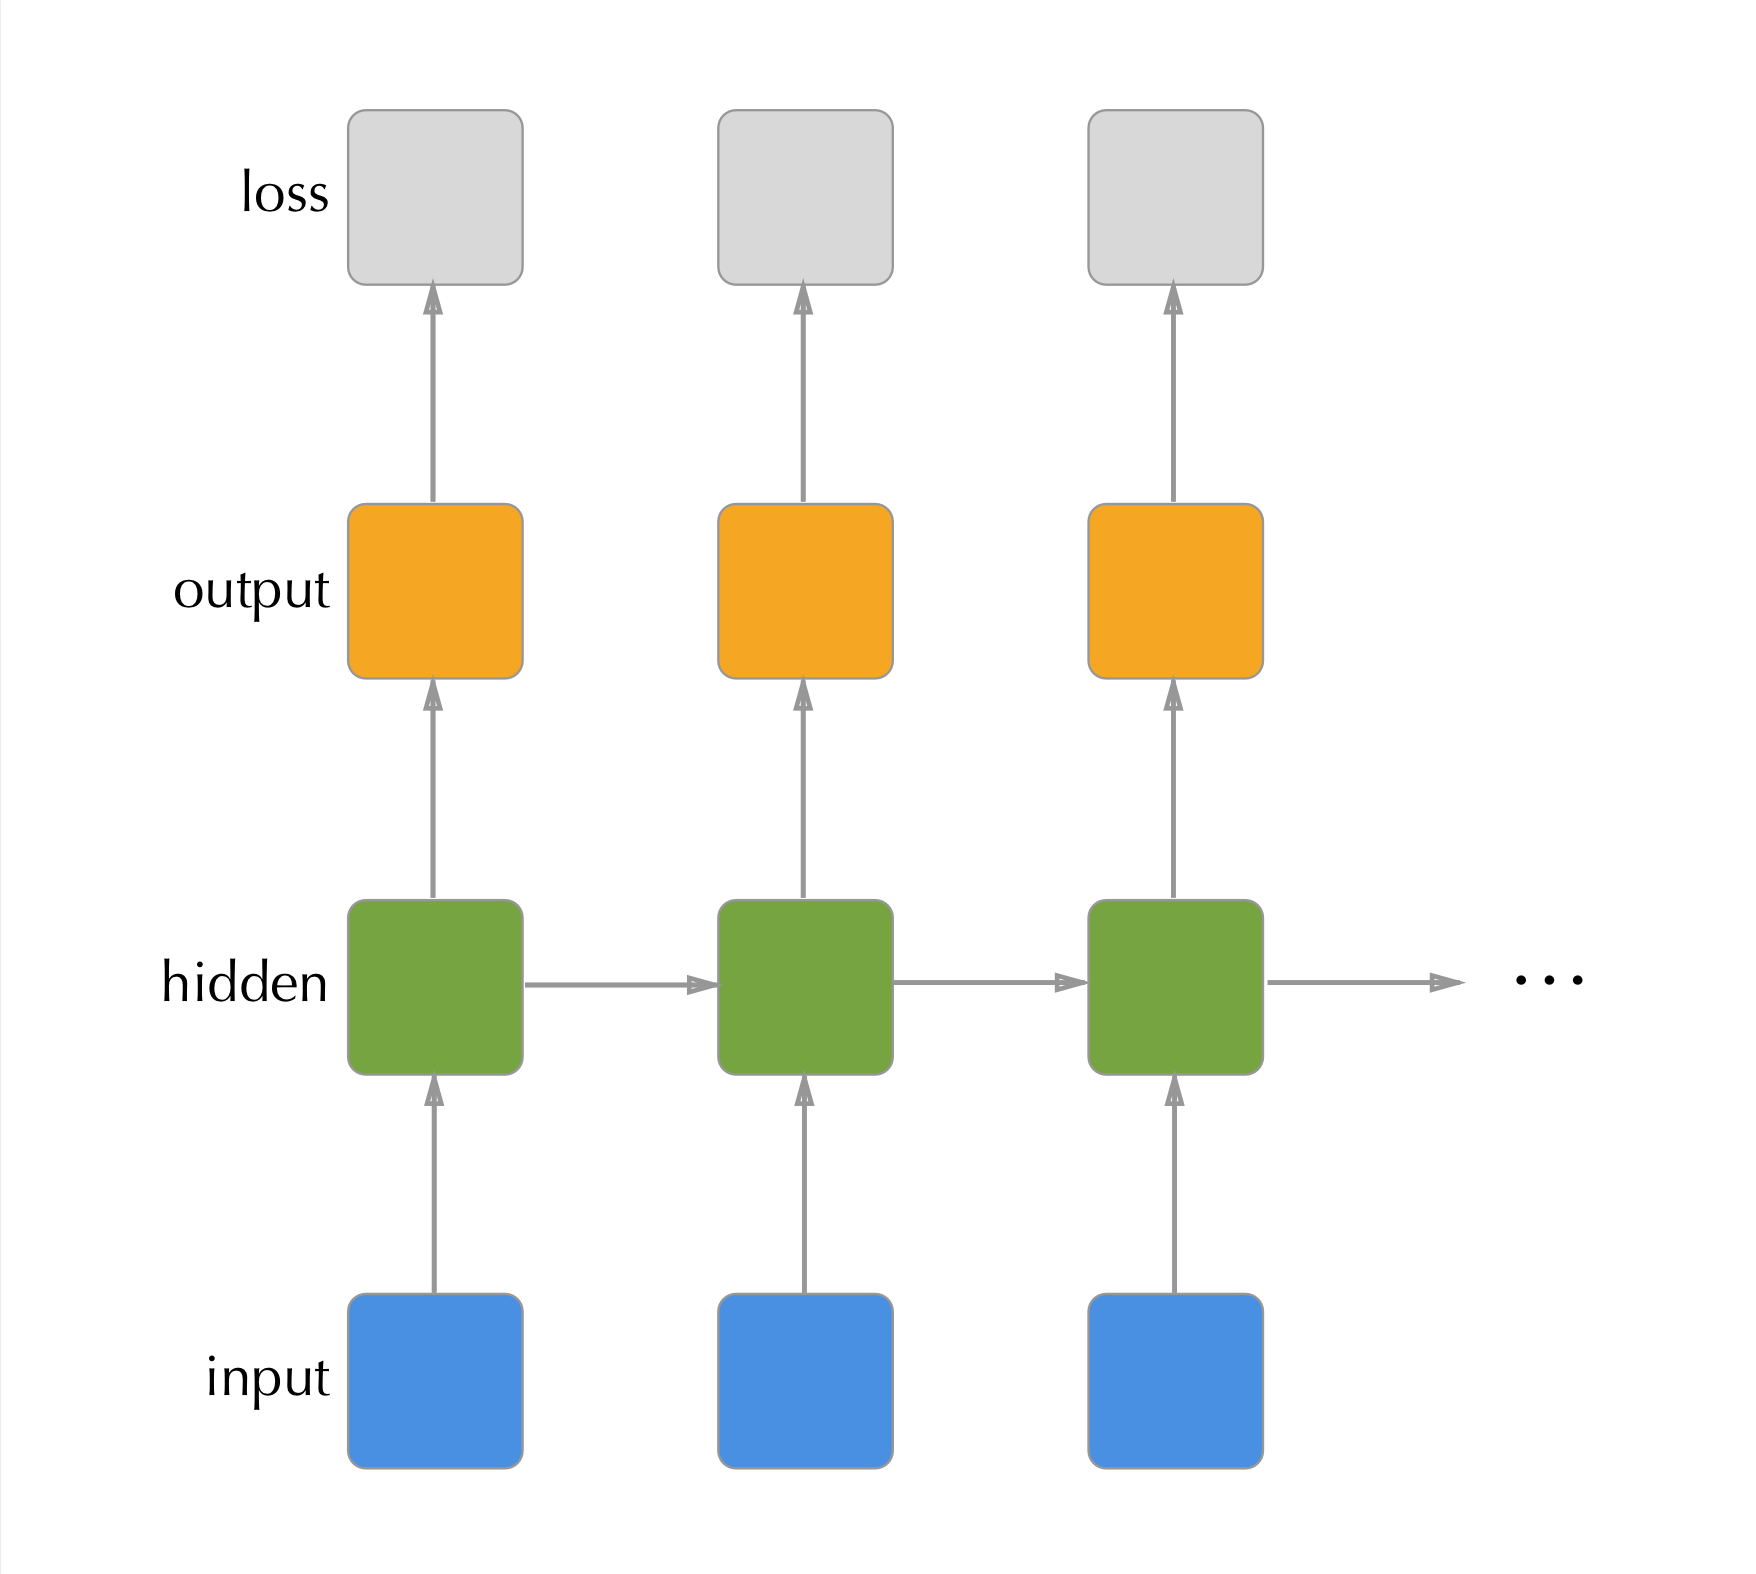
\includegraphics[width=0.65\linewidth]{figures/rnn_unrolled} 

}

\caption{Unrolled view of the RNN shown in previous figure. Each timestep has two outputs, the timesteps predictions and its hidden state. The next time step subsequently has two inputs: the data at the timepoint and the previous timepoint's hidden state.}\label{fig:unrolledgraph}
\end{figure}

So in fact, we still satisfy the requirement of a directed acyclic
computation graph, just it is convenient to represent the unique layers
in the graph in a single cyclical diagram.

\subsection{Weight sharing}\label{weight-sharing}

The unrolled graph representation shows that a recurrent neural network
is actually a very large neural network, so untuitively it should be
hard to train. The secret to RNNs having maintainable parameter
quantities is weight sharing. In the unrolled graph every layer has the
same weights. This means that the hidden layer always parses the input
data with the same affine function and combines it with the previous
hidden state in the same way; likewise, with the same hidden state
activation, the model output will always be the same\footnote{We rely on
  the model to learn a hidden state that stores information from the
  past to avoid the problems with Markov processes}.

In order to calculate gradients, first an initial hidden state is
defined (usually all zeros) and then forward propagation is carried out
through all \(t\) time-points of the input. Then, back propagation
starts from the last output and proceeds all the way back through the
computation graph. The resulting gradient descent updates are a function
of the average of all of the gradients calculated. This procedure,
although technically no different from plain back propagation, is known
as the \emph{back-propigation through time} (BPTT) algorithm. For a
thorough overview of the form of the gradient equations for BPTT see
\citet{goodfellow_DL} chapter 10.2.2.

\subsection{Problems with exploding and vanishing
gradients}\label{problems-with-exploding-and-vanishing-gradients}

One way to think of an RNN is a series of function compositions over
time. Much like a `deep' neural network is a series of function
compositions through it's layers, the unrolled computation graph of the
RNN is `deep' in time. While a traditional feed forward network
typically have somewhere between two and ten layers of this composition,
RNNs can have hundreds of steps of this composition as sequences are
commonly very long (e.g.~time series data collected every second for a
day: \(t= 86,400\)). When this many compositions are performed negative
side effects tend to accumulate. The largest being the problem of the
exploding and vanishing gradients (\citet{vanishing_gradient},
\citet{bengio_gradient}).

To illustrate this problem we can think of an extremely simple RNN. One
that has no input, a single hidden layer
\(\mathbf{h}^{(i)}, i \in \{1, ..., t\}\), and no non-linear activation
functions. We will denote the weights for mapping
\(\mathbf{h}^{(i)} \to \mathbf{h}^{(i + 1)}\) with \(\mathbf{W}\). We
also assume that \(\mathbf{W}\) can be eigendecomposed to
\(\mathbf{Q}\mathbf{\Lambda}\mathbf{Q}'\) where \(\mathbf{Q}\) is
orthogonal and \(\mathbf{\Lambda}\) is the eigen matrix. This is
obviously a functionally useless model, but it serves to illustrate our
problem.

We can think of each step of our RNN through time in terms of matrix
multiplication.

\begin{equation} 
  \mathbf{h}^{(t)} = \mathbf{W}' \mathbf{h}^{(t - 1)}
  \label{eq:simplernn1}
\end{equation}

This equation can be simplified to a function of only the weight matrix
and the first hidden state using the power method.

\begin{equation} 
  \mathbf{h}^{(t)} = \left[\mathbf{W}^t\right]' \mathbf{h}^{(0)}
  \label{eq:simplernn2}
\end{equation}

Next, we substitute the eigendecomposition of \(\mathbf{W}\).

\begin{align} 
  \mathbf{h}^{(t)} &= \left[(\mathbf{Q}\mathbf{\Lambda}\mathbf{Q})^t\right]' \mathbf{h}^{(0)} \\
                    &= \mathbf{Q}'\mathbf{\Lambda}^t \mathbf{Q} \mathbf{h}^{(0)} \\
  \label{eq:simplernn3}
\end{align}

The form of the function composition in \eqref{eq:simplernn3} allows us to
see that while the eigen matrix is continuously being raised to the
\(t\) power, it will cause its eigenvalues with magnitude greater than
one to diverge to infinity and those with magnitude less than one to
converge to zero.

This observation leads to the problem that, over any long term sequence,
our model will have a very hard time keeping track of dependencies. When
applied to back propagation this is essentially means that the gradients
associated with parameters linked to longer term dependencies will
either vanish (go to zero) or explode (go to infinity).

Due to the problems caused by this repeated function composition plain
RNNs have generally proved unable to learn dependencies longer than a
few time-steps\footnote{\citet{bengio_gradient} showed that after only
  10-20 steps the probability of successfully learning a dependency was
  effectively zero.}, and when they do, they are outweighed by those
closer in time, simply due to mathematical inconveniences and not
necessarily information importance (\citet{bengio_gradient},
\citet{graves_rnn}).

\subsection{Modern Extensions}\label{modern-extensions}

There have been many proposed solutions to solving the problems
associated with plain RNNs inability to learn long term dependencies.
Some of them focus on forcing gradient's into good behavior by
constraining them to be close to one (\citet{bounded_gradient_rnn}) and
others on adding `skip connections' between times further apart than a
single step (\citet{skip_connections}).

While these methods do successfully allow RNNs to learn longer time
dependencies, they are rather restrictive (forcing weights to have
gradients near one can slow down training and inflate importance of some
features and skip connections eliminate the benefit of the network
learning the dependency lengths on its own). Next, we will introduce two
methods to deal with the problems of learning long-term dependencies
that have gained wide-spread adoption and generally dominate the
techniques used.

\subsubsection{Long short term memory
networks}\label{long-short-term-memory-networks}

A way of controlling how an RNN keeps track of different dependencies
over time is to make that control flow part of the model itself and
allow it to be learned. This is the concept that long short term memory
(LSTM) networks (\citet{lstm_intro}) use. In the broadest sense, LSTM
networks augment the traditional RNN architecture by adding a series of
`gates' that control which parts of the hidden state are remembered and
used from time-step to time-step.

\begin{figure}

{\centering 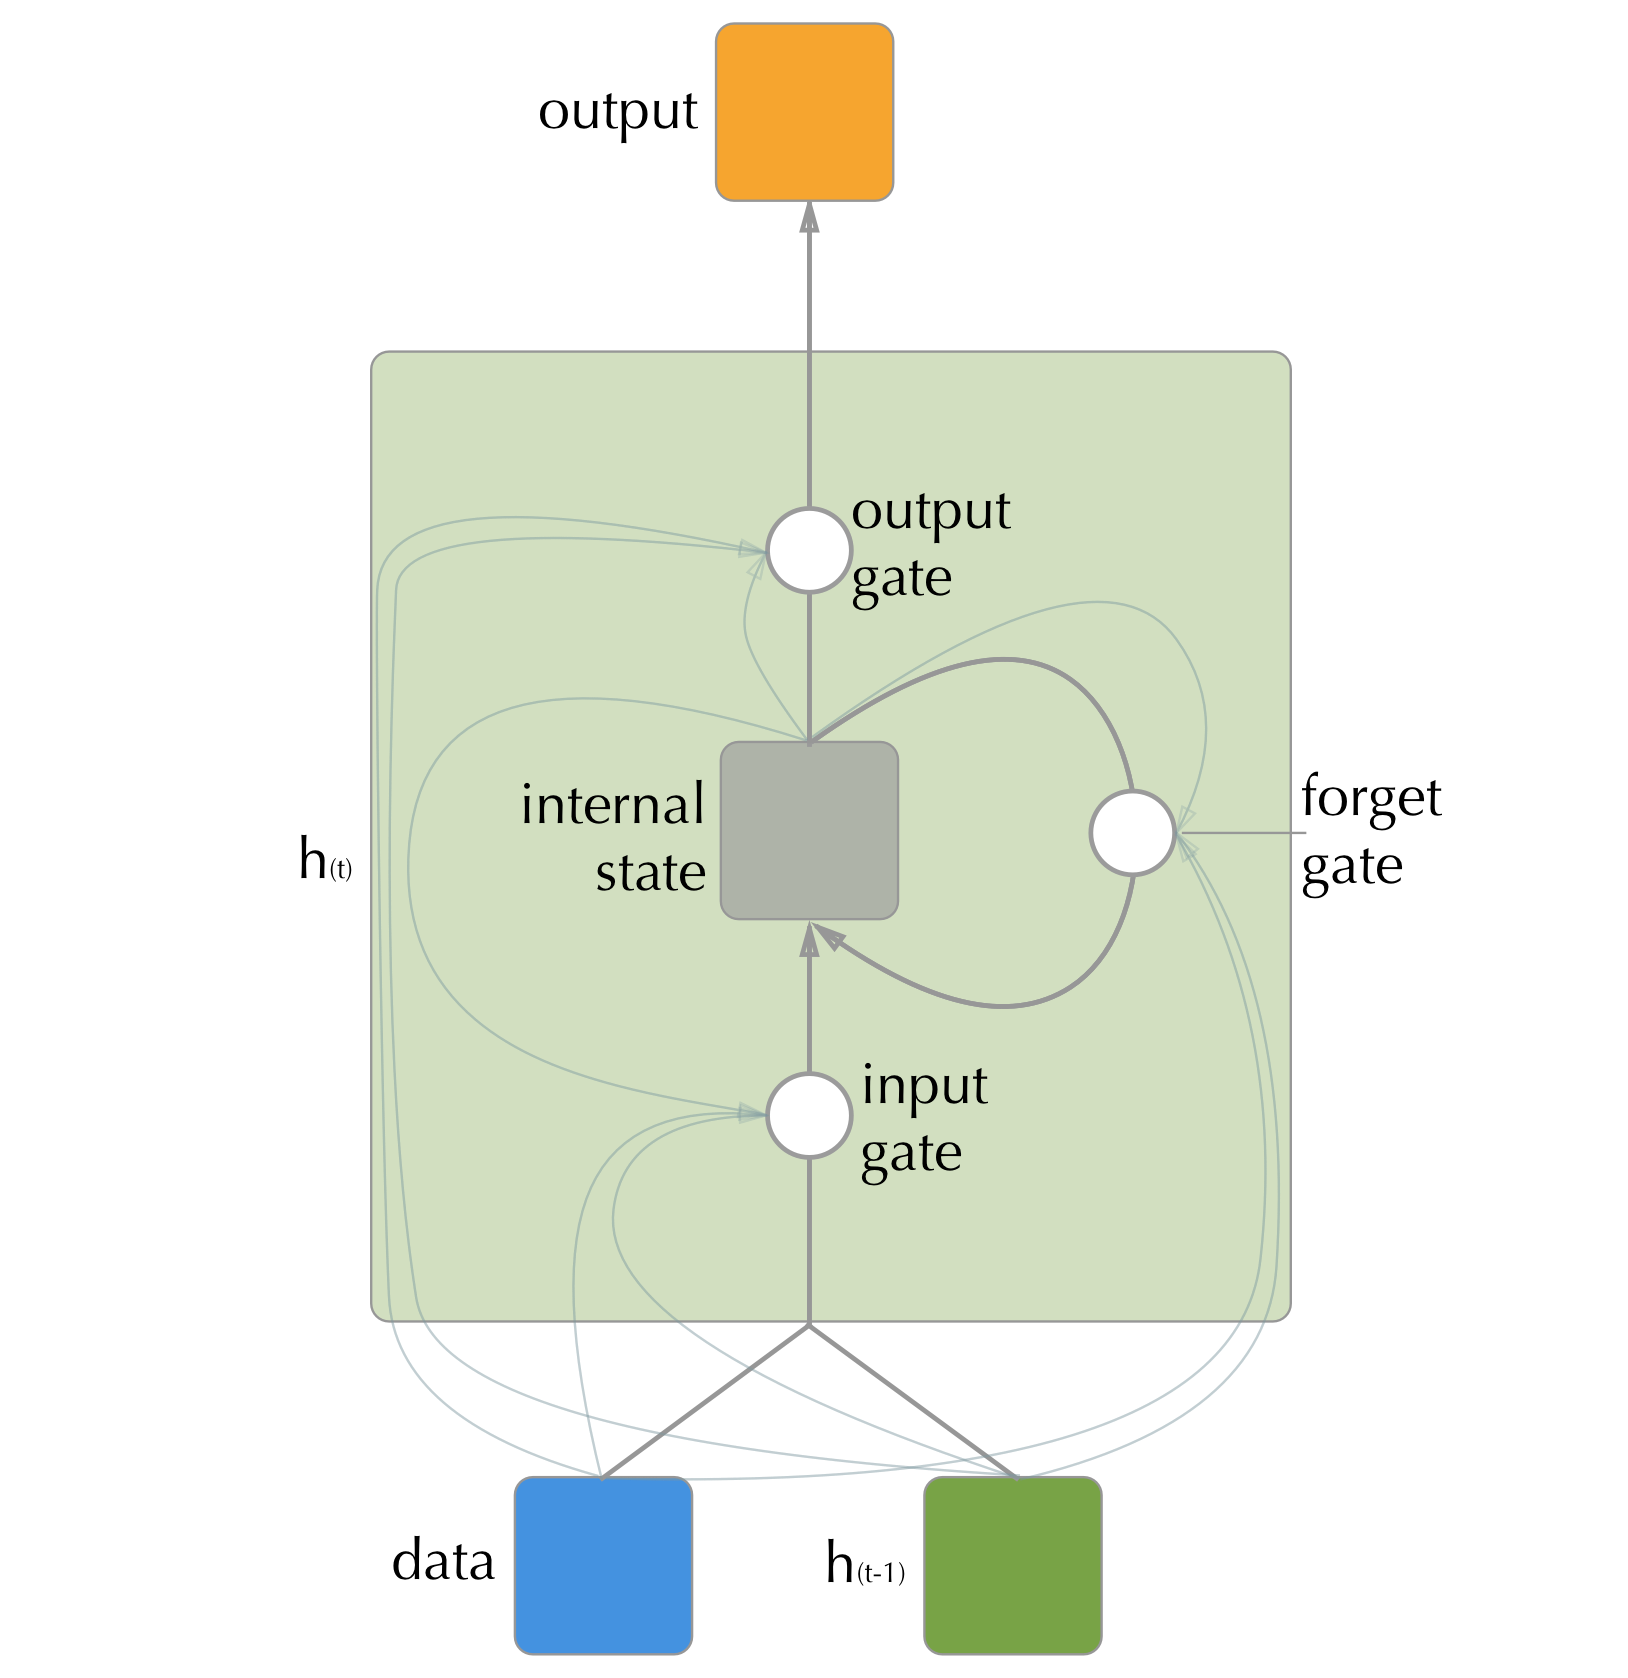
\includegraphics[width=0.6\linewidth]{figures/lstm_cell} 

}

\caption{The internal structure of an LSTM hidden unit. The gates are all fed by the input at time _t_, the whole hidden unit at time (_t - 1_), and the hidden units internal state from time (_t - 1_). The gates themselves are linear combinations of the input that are then transformed by sigmoid activation functions.}\label{fig:lstmdiagram}
\end{figure}

It is important to note that an LSTM network is really just an RNN that
has had the neurons a hidden layer replaced by a more complicated cell
that controls its inputs and outputs along with having a secondary
internal recurrence to an internal state. See figure
\ref{fig:lstmdiagram} for the details of this internal cell.

These gates are themselves neurons that take linear combinations of the
input at time \(t\), the hidden state at \((t - 1)\) and the LSTM cell's
internal state at \((t - 1)\) and produce an output that is squashed
between zero (closed) and one (open) by a sigmoid activation function.
The input gate will control what information makes it through to the
unit internal state, the forget gate decides which information from the
internal state gets recycled for the next time point, and the output
gate decides what of the internal state is important to the next layer.

While LSTMs are conceptually more complicated, their improvements in
performance over standard RNNs is drastic (\citet{lstm_intro}). The
network can now learn what features are important to its given outcome
at a given time, while at the same time filtering out information that
it finds unnecessary in context. To give intuition to this we can
imagine a baseball game. Say the batter hits a foul ball, that foul has
different implications on the outcome of the at bat depending on how
many strikes the player has when it occurred. A traditional RNN would
always choose to remember a foul the same, whereas an LSTM network could
learn this contextual frame for importance.

The major issue with LSTMs is how many parameters there are to learn.
The number of parameter's associated with a neuron in a hidden layer
jumps roughly three times over a standard RNN due to the weights
necessary for the gates. Due to this, LSTMs require a very large amount
of data to effectively train and not over-fit. In practice, these
complications, combined with the recovery of some degrees of freedom
through regularization, seem to be worth it and LSTMs are by far the
most common RNN-based architecture used today. However, some other
approaches using similar methodologies have proven successful while
reducing the number of parameters needed.

\subsubsection{Gated recurrent units}\label{gated-recurrent-units}

Introduced relatively recently (2014), Gated recurrent units
(GRU)(\citet{gru_intro}), like LSTM, use gates to help control
information flow through time, but it omits the extra recurrence step of
the internal step from the LSTM and also sets the update and forget
gates to be complements of each other, thus accomplishing the task with
a single gate. This is paired with a reset gate that controls how much
of the hidden state from the previous time-point makes it into the
hidden state's input vector.

\begin{figure}

{\centering 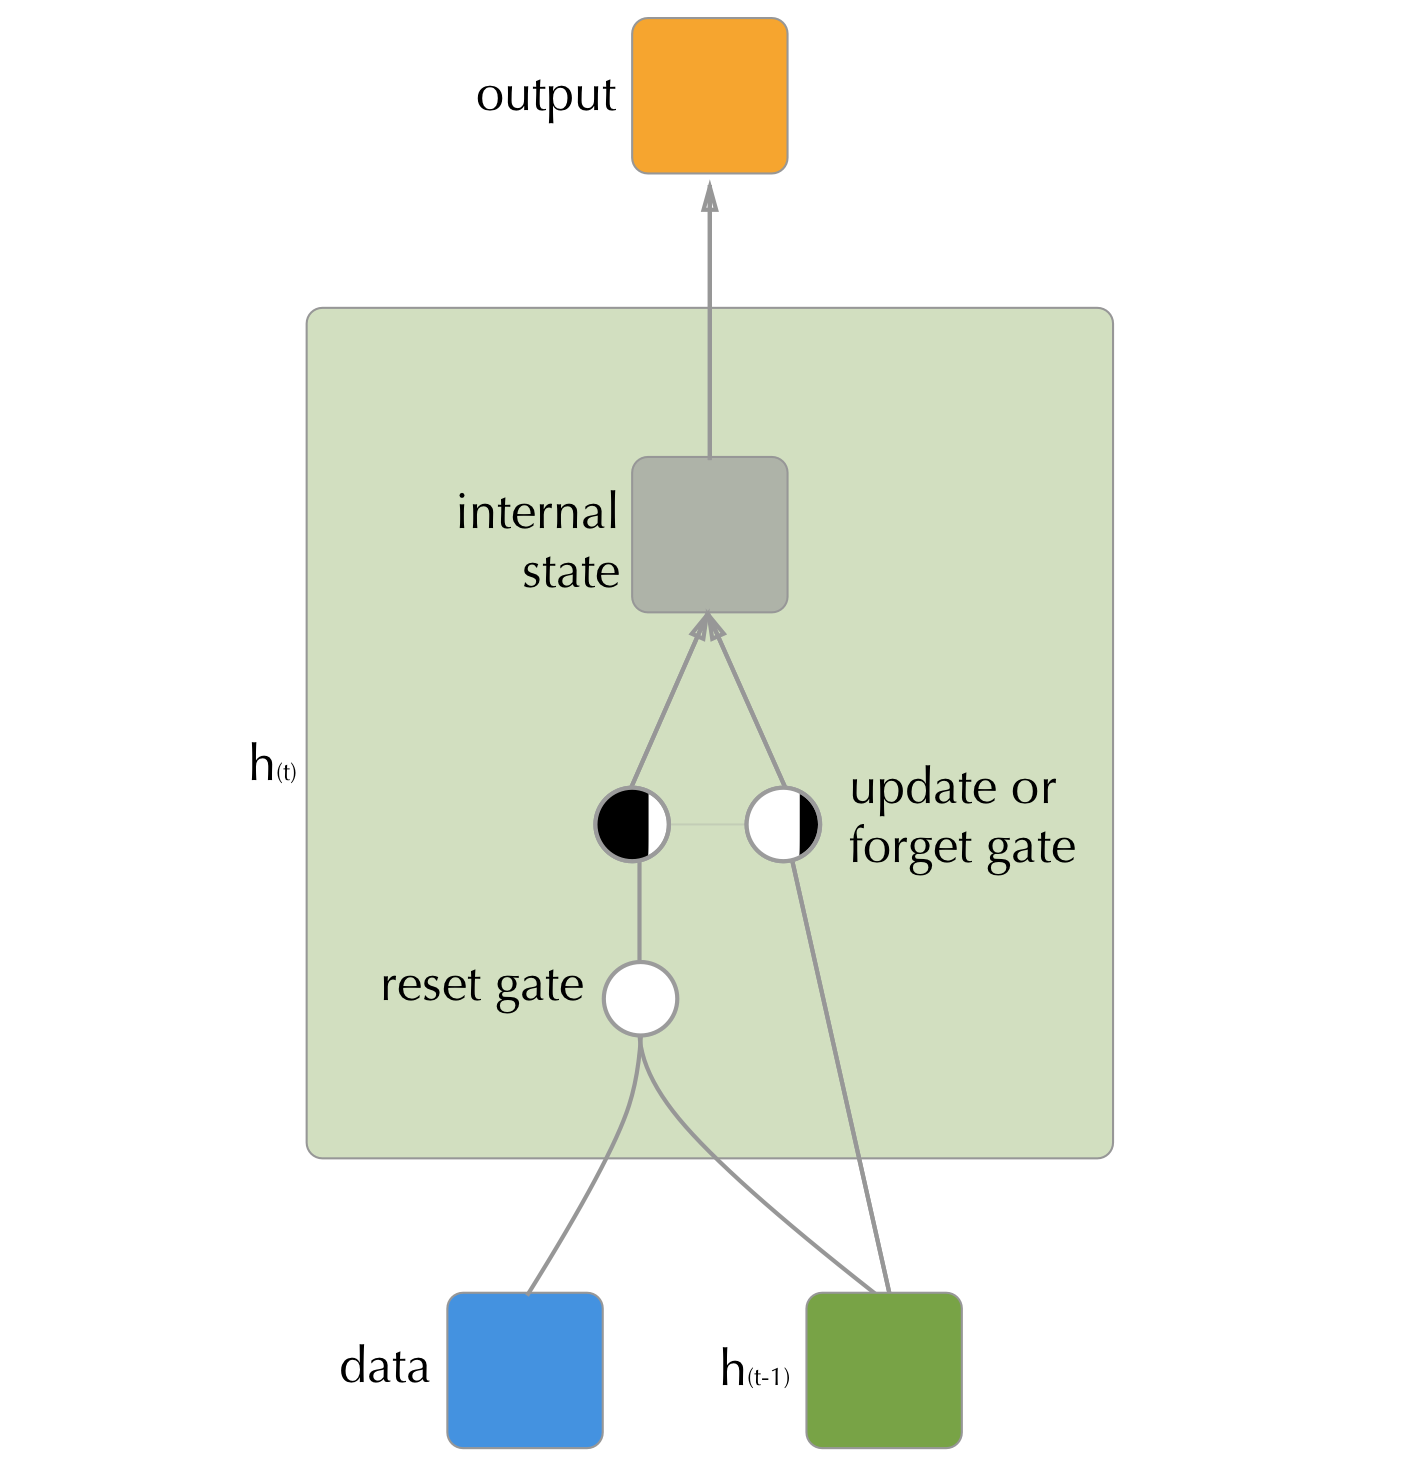
\includegraphics[width=0.6\linewidth]{figures/gru_cell} 

}

\caption{The internal structure of an GRU hidden unit. Unlike the LSTM there are only two gates, with the update and forget get tasks being taken care of by a single gate that controls what proportion to remember and what to forget. In addition, a reset gate controls how much of the hidden state from the previous step to bring into the current.}\label{fig:grudiagram}
\end{figure}

While the GRU has fewer parameters to train, and does appear to perform
better in lower data scenarios (\citet{graves_rnn}), in many cases the
increased expressiveness of the LSTM allows for better performance. A
recent large-scale survey of RNN architectures (\citet{rnn_survey})
found that on all benchmarks LSTM networks outperformed GRUs when using
a systematic hyper-parameter search.

\subsection{Computational Hurdles}\label{computational-hurdles}

The complications caused by RNNs propagating values/errors over many
time steps is also the cause of the biggest computational hurdle
associated with RNNs. When forward propagating or back propagating, we
need to do it all in one sequential set of calculations.

It is very common for neural network training to be multi-threaded using
graphics processing units (GPUs). The reason this is effective is most
of the calculations involved are simple and only depend on a few
sequential layers, and thus it is very easy to run many training samples
through the network in parallel to calculate their gradients and then
aggregate those to a gradient descent step. However, with RNNs we must
processes each sequence all the way though its (potentially very
numerous) time steps. As a result, RNNs train much slower than other
neural network architectures.

There are a few general approaches to solving this. The simplest is to
just stop back propagation at a certain number of steps, regardless of
if the sequence has been fully processed yet. This is known as truncated
back propagation through time (\citet{trunc_bptt}) and does often
substantially speed up training, but at the obvious cost of limiting the
length of time the network is able to look back in.

Another technique is to modify the architecture of the RNN such that the
hidden state receives input not from itself at the previous time point
but the output at the previous time-point. This allows the model to be
trained one time point at a time because the output from the next time
step can be substituted with the observed value at that time step. While
this approach massively speeds up training, as mentioned previously, it
throws away some potentially valuable latent-space information that the
model has learned. This approach has gained very little traction due to
these limitations.

\begin{figure}

{\centering 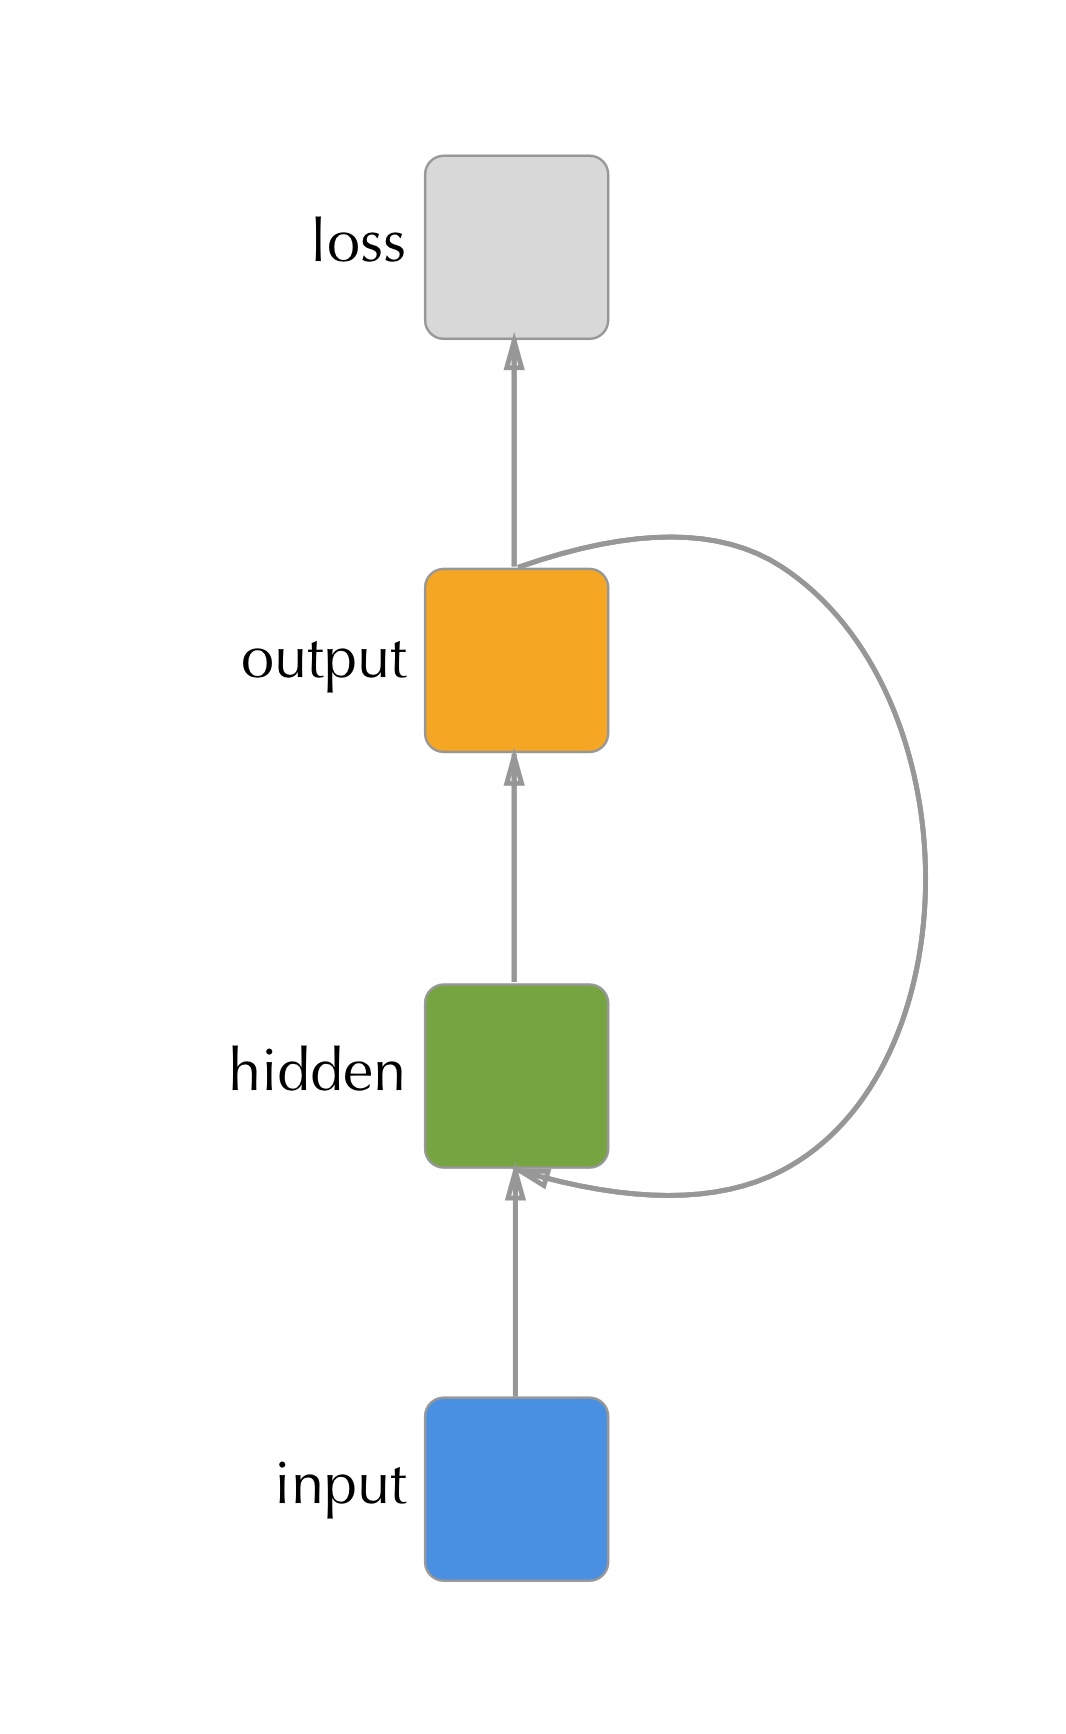
\includegraphics[width=0.45\linewidth]{figures/output_rnn} 

}

\caption{An RNN where the recurrent connection is made between the previous timepoint's output and the hidden unit. This model is less expressive than the traditional hidden - hidden architecture but is much easier to train.}\label{fig:outputrnn}
\end{figure}

As both the number of observations as well as the number of time points
grows the RNN architecture becomes increasingly strained and researchers
have begun looking at other potential ways of modeling sequential data
that allow for dynamic learning of temporal dependencies while training
in reasonable amounts of time. The most promising approach thus far has
been using convolutional neural networks.

\section{Convolutional Neural
Networks}\label{convolutional-neural-networks}

While CNNs have garnered a great amount of attention in recent years for
their successes in computer-vision they were originally introduced as a
method for modeling time-series data (\citet{hinton_cnn}){[}\^{}Although
at the time they were called time-delay neural networks.{]}. A
convolutional neural network is one where a convolution (, or window
that detects features such as edges,) is run over the spatially
connected dimensions of the data in order create a map where a given
feature is located.

\subsection{Application to spatially correlated
data}\label{application-to-spatially-correlated-data}

In the context of image recognition this mapping means scanning a
two-dimensional block of pixels over the range of the picture to detect
important features in the data. In time-series data this window is one
dimensional (e.g.~a five minute window) and it scans exclusively along
the sequence detecting some feature.

\subsection{Feature Learning}\label{feature-learning}

The power of neural networks comes in with the fact that these feature
recognizers are learned. This is in contrast with traditional approaches
where the features to be extracted had to be manually curated. Usually
some number of convolution's are initialized for a given model and are
allowed to learn the patterns that help them best minimize the loss
function. Interestingly, in the case of computer-vision, sometimes
fascinating patterns are learned that mimic what one might expect, but
are much more complicated than those manually created by humans
(\citet{cnn_vis}).

Neuroscience research has shown that CNNs mimic how the first stages of
the animal visual perception system works (\citet{cnn_animals}) and has
in many cases surpassed human level performance on basic tasks.

\begin{figure}

{\centering 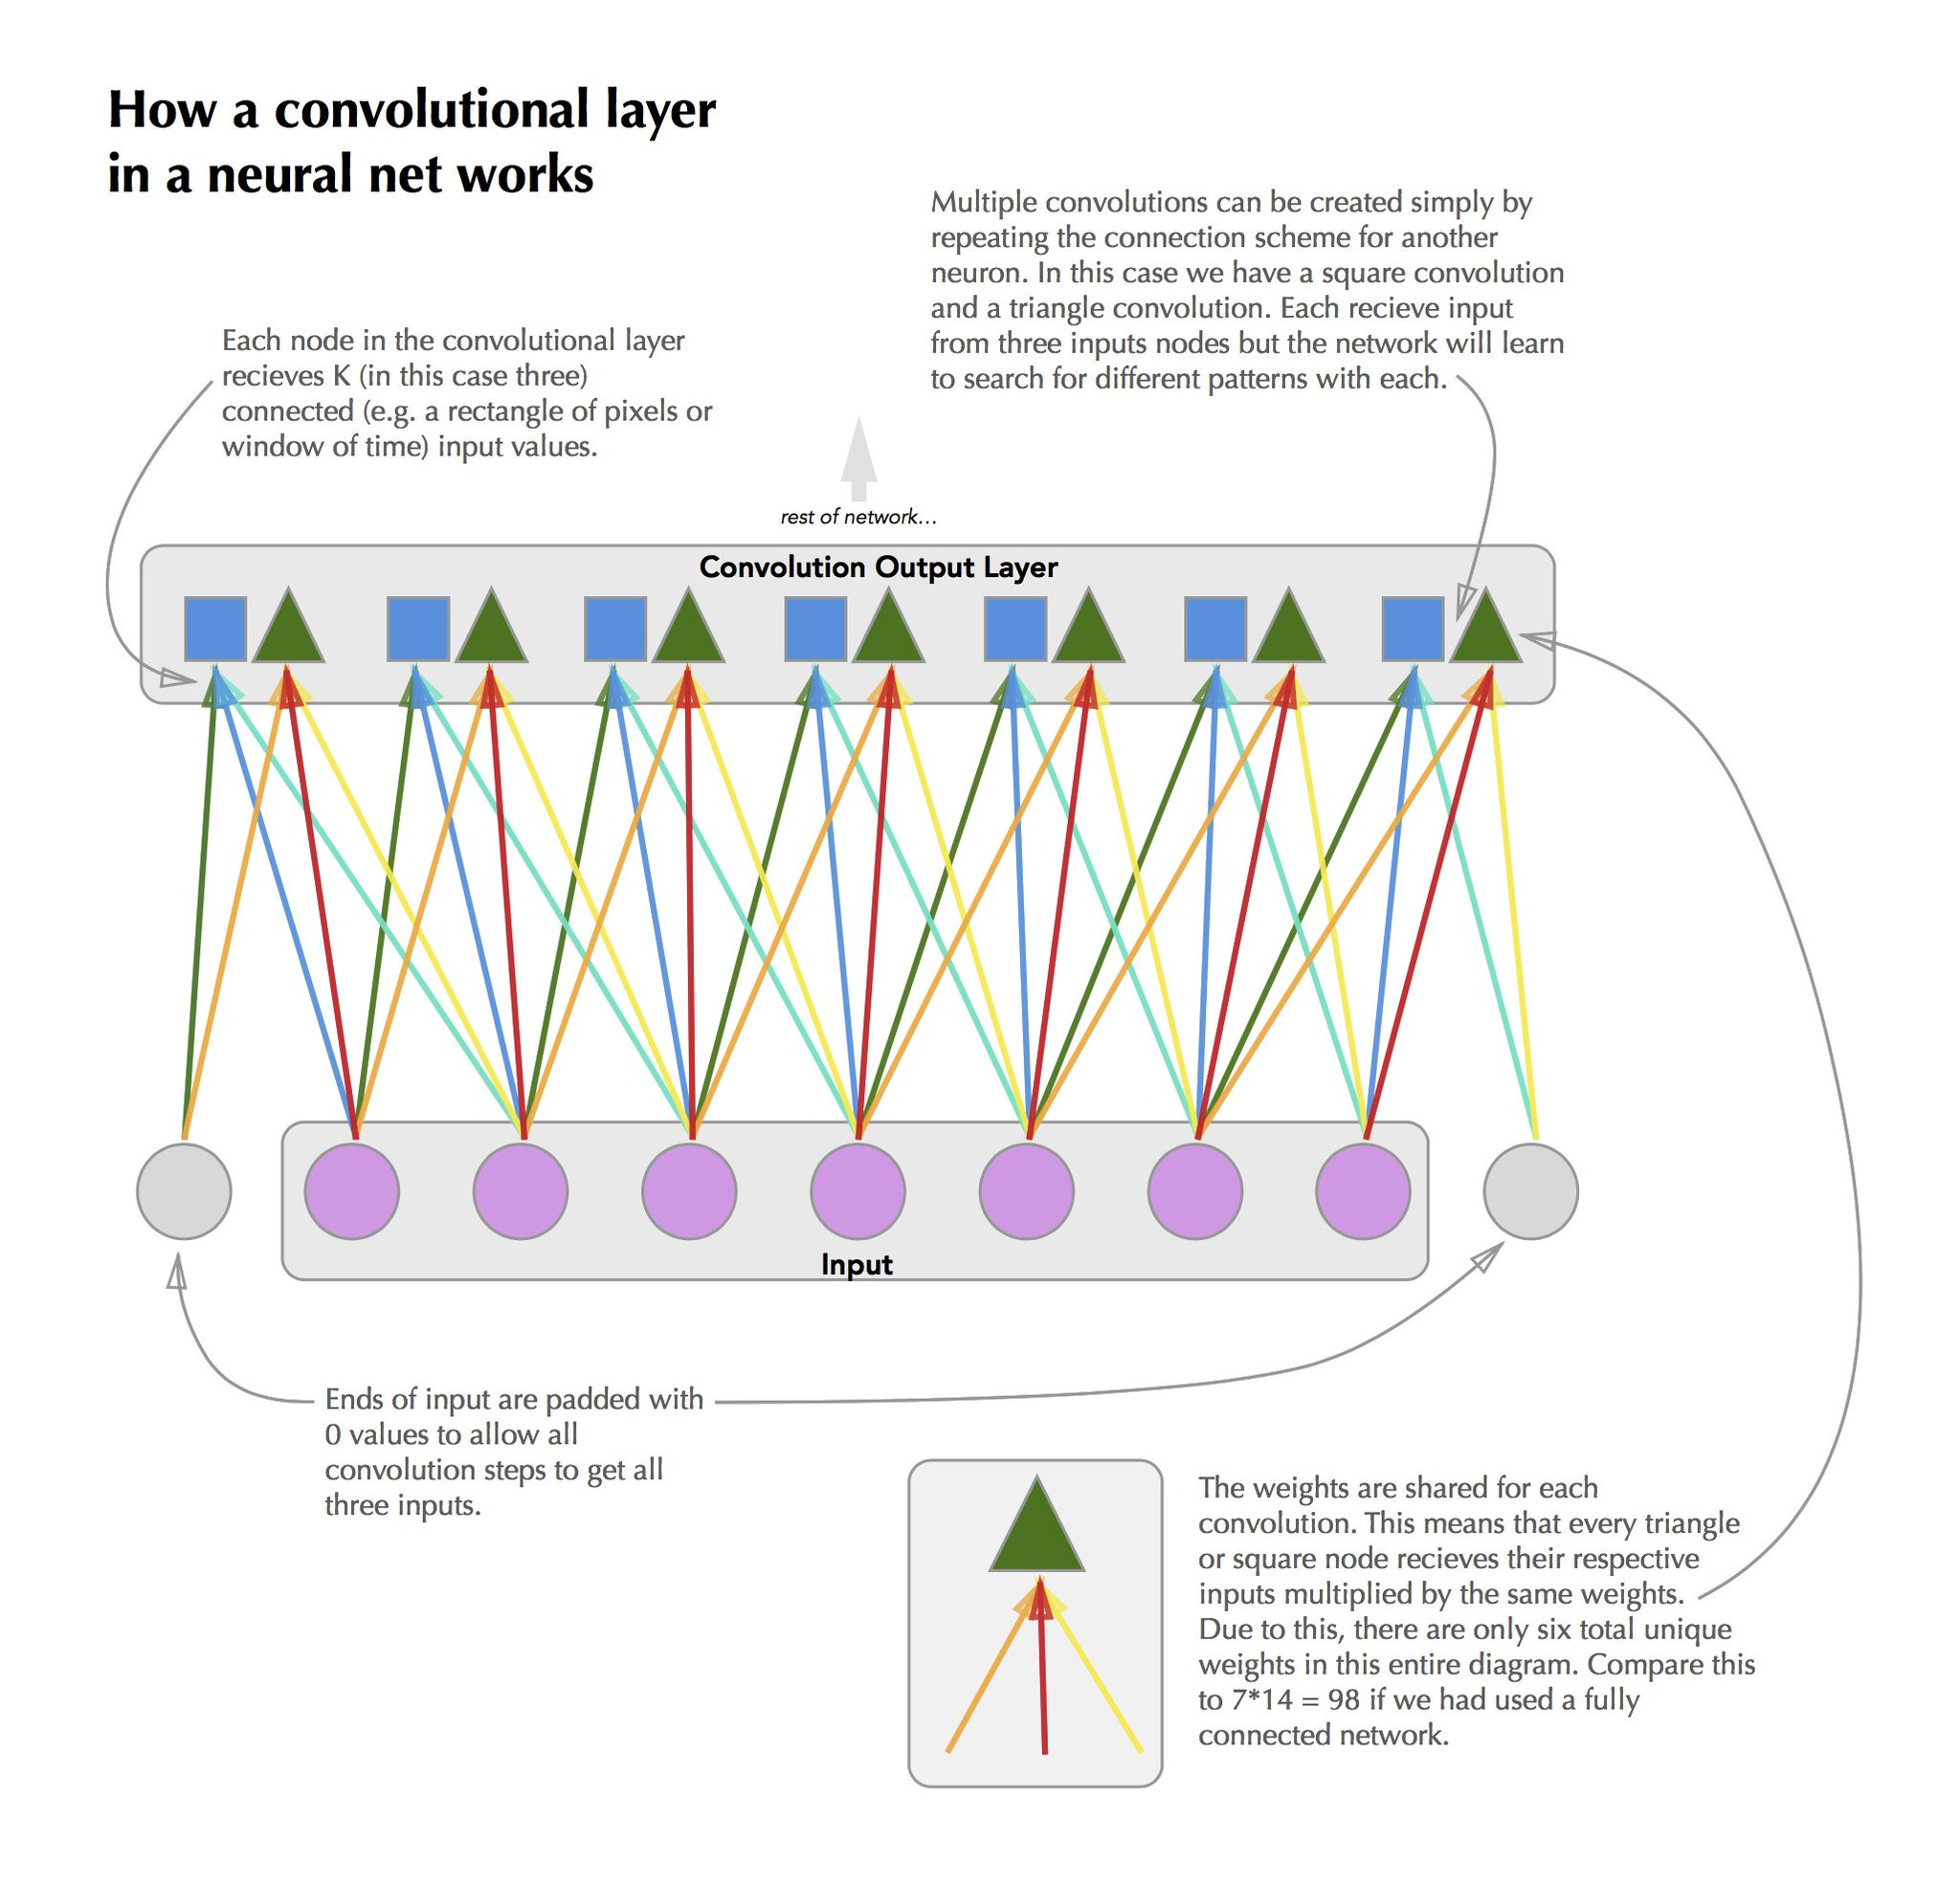
\includegraphics[width=1\linewidth]{figures/convolutional_explainer} 

}

\caption{A diagram of how a convolutions are applied to sequential data.}\label{fig:cnnexplain}
\end{figure}

\subsection{Weight sharing}\label{weight-sharing-1}

Like RNNs, a CNN can be thought of in the context of a traditional feed
forward neural network. A convolution operation is simply the sharing of
weights between grouped blocks of the hidden layers. For instance, if we
had two convolutions of length three that were reading in sequential
data in the hidden layer neurons (1,2,3) would correspond to convolution
one on the first time-point of the input, neurons (4,5,6) would
correspond to convolution two on the first time point, neurons (7,8,9)
to convolution one on time-point two, and so on. See
\ref{fig:cnnexplain} for a visual treatment of this\footnote{The actual
  location placement of the convolutional outputs for the next layer
  does not actually matter unless the next layer is itself a
  convolutional layer.}.

\subsection{Translation invariance}\label{translation-invariance}

After the first convolutional layer has produced a map of the location
of certain features on the input, subsequent layers can perform what is
known as a `pooling' operation to both reduce the dimensionality of the
latent space and also to make the feature detection translation
invariant.

A pooling layer acts similarly to a convolutional layer in that it scans
sequentially over its input, however in the case of a pooling layer the
input is the output of a convolutional layer. In addition, instead of
applying some learned linear transformation to its inputs, it performs a
predesignated pooling operation such as finding the maximum, or average
of the input values for its window and then returning that singular
value. By taking steps larger than one between each application of the
filter (also known as the stride), this serves to create an indicator
for if a feature was `seen' in the region, but it does not care about
where in that region it was seen.

This can be beneficial in many scenarios. For instance, if you were
trying to identify the waveform of the word ``dog'', one feature
detector may be to find the pattern corresponding to the ``d'' phoneme,
and one to the ``au'' phoneme. Depending on the speed of the speaker,
the ``d'' phoneme might appear two tenths of a second before the ``au''
one or one tenth. By pooling we help the model getting confused in this
case, because it just looks for the ``au'' phoneme to occur in a
flexible window after the ``d'' one.

Translation invariance does also have its downsides too. Geoffrey Hinton
(coincidentally the inventor of CNNs) has been very open about how he
thinks
\href{www.youtube.com\%2Fwatch\%3Fv\%3DrTawFwUvnLE\&usg=AOvVaw3CKtrHEhfBZkXdd7xgJ1PM}{they
are bad models}. His main complaint rests with the fact that pooling
layers throw away large chunks of information in ways that animal vision
systems do not. Recently he published a paper with co-authors Sara
Sabour and Nicholas Frosst that introduces a new architecture called the
``capsule network'' (\citet{capsnet}) which acts similarly to a
convolutional network with pooling, but it preserves information about
the translation of the feature.

\chapter{Opportunities for advancing field}\label{future}

Up to now has been an overview of the techniques in deep learning that
have been successfully and commonly implemented in sequential
classification problems. This chapter will be devoted to new efforts of
solving problems associated with the aforementioned methods. In addition
to being a survey of the current state of the art it will also identify
potential avenues for new research that could enhance our ability to
work with sequential data subjected to various constraints.

\section{What to do with all those
parameters}\label{what-to-do-with-all-those-parameters}

An issue with not just sequence-based deep learning, but the field as a
whole, is how large models are. For instance: VGGnet (\citet{vggnet}),
the second place winner of the 2014 ImageNet competition and an
extremely common model to use for image recognition tasks, has 138
million parameters to tune. Going by the rule of thumb from Frank
Harrell's book ``Regression Modeling Strategies'' (\citet{rms}) of 10-20
observations per parameter in our model, this is an issue, especially
given the size of the data-set that the VGGnet model was trained on was
\emph{only} one million images\footnote{This comparison is not exactly
  fair as images are composed of many pixels as well.}.

Even simple neural nets have a large number of parameters. A model with
just a single hidden layer taking a ten dimensional input and a hidden
layer of ten neurons performing binary classification would have (with
bias parameters included) \((10*11) + (10*11) + (2*11) = 242\)
parameters to tune.

\subsection{Theory backed methods for choosing model
architectures}\label{theory-backed-methods-for-choosing-model-architectures}

How then, did the VGGnet model achieve an accuracy of 93\% on the test
set? The answer lies in the fact that data is not shared over parameters
in the same way it is in regression models. This stems from the fact
that each layer's parameters are using as their input the output from
the previous layer, and thus data are being reused. While it does not
appear that this means we only need to count the parameters in the first
layer, it does mean that deep learning models need to be thought of
differently than traditional regression based models in terms of
parameter complexity\citep[\^{}It also points to the advantages of deep
neural nets over wide ones, a topic considered more deeply in][ chapter
13.]{goodfellow_DL}.

As of yet, there is no solid theoretical explanation of exactly what the
data to parameter relationships are in deep neural networks, and thus
there are no concrete guidelines to model construction. Difficulties in
ascertaining these guidelines seems in part due to the non-convex
optimization routines used for the models.

The combination of the lack of theory and the computational time needed
to perform traditional grid-search techniques for tuning layer
numbers/size suggest the potential for very impactful research in this
area.

\subsection{Runtime on mobile
hardware}\label{runtime-on-mobile-hardware}

Another impact of having extremely large models is they take a long time
to not only train, but to be used to predict as well. If deep learning
models are to be brought to mobile devices such as smart phones or
watches the models need to be scaled down in terms of their size and run
time complexity substantially. Efforts towards this have been successful
with models such as SqueezeNet (\citet{squeezenet}) drastically reducing
the number of parameters compared to traditional convolutional networks,
while still maintaining a good level of accuracy in ImageNet prediction
performance. In addition, certain forms of penalization such as \(L_0\)
penalization can be applied to `thin out' a network by forcing certain
weights to drop to zero and then throwing them out (\citet{sparsenets}),
all while performing a single run of stochastic gradient descent,
eliminating the need to do costly re-training of the network after
dropping weights.

Great opportunity lies the development of objective and rigorous methods
of eliminating unnecessary parameters in models. Approaches such as
regularization are promising as are the evaluation of model response to
techniques such as dropout (\citet{dropout}) where by neurons are
randomly dropped during forward propigation in training in an effort to
build robust prediction pathways. An analysis of a model's response to
certain neuron's being dropped may indicate the potential for sparsity
inducing techniques.

\section{Inference}\label{inference}

A great source of confusion for many statisticians when reading
literature in the deep learning world is that in many cases the same
words have different meanings. ``Inference'' is a good example of this.
To a statistician inference means the dissection of the inner workings
of the model: what parameters are used to make predictions and how
confident are we in those parameters. In deep learning, inference
typically refers to the use of a model for prediction. There are a few
things that stand in the way of traditional inference in deep learning
models.

\subsection{Peering into the black
box}\label{peering-into-the-black-box}

Often it is common to hear people refer to deep neural networks as
``black box predictors.'' This meaning simply that data goes in and the
model performs some uninterpretable transformations to that data and
returns its prediction. While in giant models such as VGGnet may make
this seem like the case, it is actually quite possible to see what is
going on within a neural network, just the quantity of information to
understand is too high to fully comprehend it in its raw form.

The desire for traditional inference in the statistical sense is a
limiting goal. Having a parameter estimate and its uncertainty works
well when models are single-stage linear combinations of the data, but
neural networks, and arguably the world, does not usually work in linear
combinations. Traditional inference has relied on making (hopefully)
non-impactful simplifications of the true nature of the system being
modeled in order for it to fit the framework of linear models.

With deep learning we have a system theoretically capable of modeling
any function of data and we should take advantage of that. If the model
objectively performs well, we should perform the simplification on the
explanation side, rather than the model side. How exactly this is done
is not a solved issue (and may never be), but some early examples
include the work of visualizing the intermediate layers in computer
vision models (\citet{cnn_vis}): investigating the features learned by
neural networks can provide great insight into the way it parsing the
signals in the data.

\subsection{Generative Adversarial
Networks}\label{generative-adversarial-networks}

One approach that allows simultaneously attempting to train a better
model, but also understanding the workings of the model is a class of
deep learning models called ``generative adversarial networks'' (or
GANs)(\citet{gans}). GANs train two separate neural networks in tandem:
a generator and a discriminator. The job is for the generator to
construct fake examples of some training set and the discriminator's job
is to decide if the example is a real observation or a generated one.
These models have shown remarkable results in terms of image generation
such as those recently presented by NVIDIA \ref{fig:ganexample}
(\citet{progressive_gans}).

\begin{figure}

{\centering 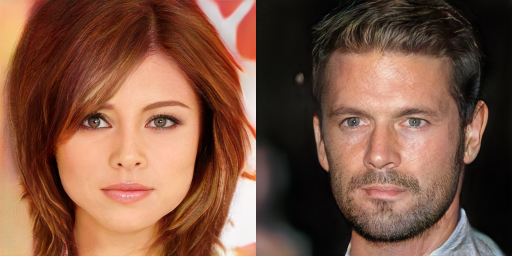
\includegraphics[width=0.8\linewidth]{figures/gan_example} 

}

\caption{The output of a generative adversarial network trained on a database of celebrity faces. Both faces seen are entirely generated by the model and show that it learned to a very precise degree, what constitutes a 'face.'}\label{fig:ganexample}
\end{figure}

The output produced by the generator model of GANs effectively show what
the descriminator model is `seeing' when it chooses to classify
something as a given class. For instance, an over-fit model may classify
a house as a house because it sees a lot of the color blue in the sky.
If that was the case a GAN would simply return a blue canvas when asked
to generate a house\footnote{Another similar approach is neural networks
  with `attention' mechanisms (\citet{attention}). These mechanisms can
  be used to explore what exactly in the data is contributing heavily to
  a given classification.}.

Recently, a team at ETH Zurich used GANs on time series data taken from
hospital records (\citet{medical_gans}) and found that GANs could be
used successfully on these data to generate realistic looking medical
data, suggesting that the model was learning underlying patterns
well\footnote{This opens a fascinating ethical conundrum in that,
  theoretically if over-fit, the model could serve to simple memorize
  patient data and would be a serious privacy threat. How do we decide
  when the model is interpreting general trends and when it's working on
  the individual level? Are there cases for both?}.

\subsection{Causality problems}\label{causality-problems}

While much of deep learning is not currently focused on uncovering
causal pathways\footnote{It is being explored however, particularly in
  the Bayesian deep learning communities.}, given the ability of these
models to generalize so well, it is worth exploring the issue more. One
area of concern with the models mentioned is the temporal order of data.
For instance, in convolutional methods for sequence classification,
often the convolutions are allowed to explore not only back in time, but
also forward in time to classify at a given instance. The same goes with
a class of RNNs that we didn't discuss but have proved successful: the
bi-directional RNN. In this case the RNN's hidden state path travels not
only forward in time, but also backwards.

These models that can see both backward and forward in time often
perform better than their omni-directional counterparts. For instance,
in speech the ``au'' phoneme may indicate an `e' or an `a' in a word,
but it only becomes clear after the end of the word is heard which value
it is. However, the flow of causality is forward in time, so these
models explicitly violate this.

Potentially fitting a model that has the ability to see both forward and
reverse temporal dependencies and then investigating the dependencies
that were discovered by both directions could provide some insight into
this. For instance, if the backwards in time component of the RNN found
that the administration of some drug was a strong signal that high
blood-pressure would later occur, but not the reverse direction the
relationship could warrant further experimental exploration of causality
potential. It would be necessary to make sure that the patterns
discovered were not due to residuals from the reverse-time predictors,
but this could be done by forcing the model to `forget' those patterns
and seeing if our forward-time trends remain.

\section{Small or sparse data}\label{small-or-sparse-data}

Deep learning has come to be almost synonymous with `big data.' Most of
the groundbreaking work tends to come out of large companies with
massive data-sets and near-infinite compute power to fit their models.
This has left the area of deep learning corresponding to small data
relatively unexplored. We have already seen that deep learning models
seem to use their parameters more efficiently than traditional
statistical methods, but that is clearly not without limit. The
following are a brief survey of a few techniques for dealing with small
or sparse (meaning a large portion missing labels) data.

\subsection{Bayesian deep learning}\label{bayesian-deep-learning}

As we have seen, a neural network is essentially a series of stacked
linear models with static non-linear transformations applied. Much like
we can fit a regression model in a Bayesian context, we can fit a deep
neural network with Bayesian techniques. To do so, each tuneable
parameter is simply provided a prior (usually a normal centered at zero)
distribution and the posterior distribution is determined the same as
any other Bayesian model. Usually variational inference techniques are
used instead of sampling techniques such as Hamiltonian Monte Carlo due
to the size of the models (\citet{bayesnets}).

Bayesian neural networks have been shown to perform more efficiently on
small data-sets than traditional models (\citet{dropout}). In addition,
some generative models such as autoencoders (see section below) have
shown subjectively better results from Bayesian implementations than
standard implementations (\citet{variational_autoencoders}).

\subsection{Semi-supervised methods}\label{semi-supervised-methods}

In many circumstances the data may not be small as a whole, but the
number of observations that have labels for the desired prediction are.
An example of this is activity tagging data. For each day twenty four
hours of time-series data are gathered on the subject, but often when
asked to tag the data they only tag specific instances of activities,
leaving much of the day blank. In addition it is often infeasible to ask
them to label every day of their data.

Another example comes from EHR based studies. Many times these studies
rely on using physicians to perform chart reviews in order to construct
their training and test sets. This is a costly and time consuming
procedure.

\begin{figure}

{\centering 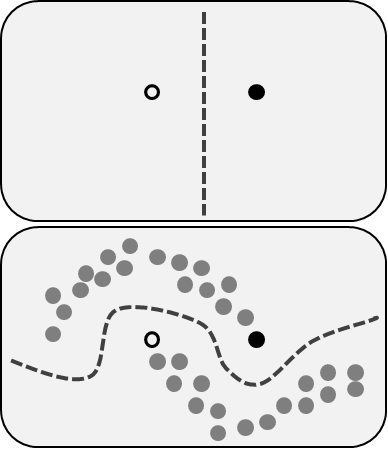
\includegraphics[width=0.4\linewidth]{figures/semi-supervised} 

}

\caption{Visual example of how adding unlabeled data can provide valuable information about the shape of the data valuable for classification. Image taken from [Wikipedia](https://en.wikipedia.org/wiki/Semi-supervised_learning)}\label{fig:semisupervised}
\end{figure}

There are various approaches to dealing with this sparse data issue. A
very promising avenue is the preliminary fitting of an unsupervised
model on the data, followed by a supervised learning model using
features learned by the unsupervised model

Say we wished to classify sentiment of a corpus of text, but only had
labels of sentiment for a small subsection of the text. First an
unsupervised model would be fit to all of the data. For instance a model
trained to predict the next word in a sentence. This unsupervised model
would learn to map the text at a given time-point to some latent-space
that holds information about the next word and most likely sentiment as
well. Tthe final layer of the word prediction model that maps that
latent-space to the next word is removed and replaced with a new layer
that fits the form of our desired classification (in this case a binary
outcome of ``happy'' or not). This new model is then trained on the
labeled data with the weights of the lower-layers either frozen at their
values from the unsupervised step or simply initialized at them.

This approach of unsupervised pre-training has been shown to yield great
improvements in the performance of sequence models
(\citet{semi_supervised}).

Other methods of performing semi-supervised learning include training
the model on available labels, then using the trained model to classify
the unlabeled data and then retraining the model treating those labels
as the true values. Surprisingly this method does almost always yield
improvements over not using any unlabeled data(\citet{semi_supervised}).

Exploration of the operating characteristics of semi-supervised learning
scenarios could be a valuable contribution to areas of research such as
electronic health records. An example of potential impact: a pseudo
power calculation could be performed at the outset of a modeling effort.
This would help the researchers optimize time and money by informing how
many labeled examples needed to be collected. In addition, efforts to
extend the performance benefits of semi-supervised learning could allow
models to be fit to domains where they were previously not able to be
due to difficulties in gathering labels for data.

\bibliography{book.bib,packages.bib}


\end{document}
